\documentclass[14pt, a4paper]{book}
\usepackage[utf8]{inputenc}
\usepackage[T1]{fontenc}
\usepackage[margin=1in,marginpar=0.75in]{geometry} 
\usepackage{amsmath,amsthm,amssymb,amsfonts, fancyhdr, color, comment, graphicx, environ, bm}
%\usepackage{xcolor}
%\usepackage{mdframed}
\usepackage[shortlabels]{enumitem}
%\usepackage{indentfirst}
%\usepackage{simpler-wick}
\usepackage{booktabs}
%\usepackage{siunitx}
\usepackage{physics}
%\usepackage{polynom}
%\usepackage{verbatim}
%\usepackage{tensor}
\usepackage{todonotes}
%\usepackage{dcolumn}% Align table columns on decimal point
\usepackage{listings}
\usepackage{caption}
\usepackage{subcaption}
\usepackage[backend = biber, style = vancouver]{biblatex}
\bibliography{refs.bib}
\usepackage{hyperref}
\hypersetup{
    colorlinks=true,
    linkcolor=blue,
    filecolor=magenta,      
    urlcolor=cyan,
    citecolor=cyan,
    % pdftitle={../Model_independent_search_for_Dark_Matter},
    %pdfpagemode=FullScreen,
    }

\usepackage{subfiles} 

\begin{document}

\graphicspath{{../../figures/}}
\section{Data Preparation/LOG}
We are dropping $\Delta\Phi(l_1,l_2)$ and $\Delta\Phi(l_c,E_T^{miss})$ due poor overenstemmelse with data. The first one is most likely due us not including fake leptons (and also for all non SFOS final states). The latter is a problem that PhD. Even is being haunted by. There is also the problem of missing variables. For the dataset being used I only look at, at least, two jets in the final state. This does however not always happen, to "fill the gaps" I made the $p_T$ of the jets equal to zero if there are less than two events, which is physically reasonable. And more problematic, I set the $\eta$ and $\phi$ to 10, which has no physical meaning. Luckily this does not seem to be an important feature when training the network using XGBoost. There is also another problem, albeit less problematic than the previous ones, with the final states that are not SFOS, as the background on these tend to be lower than the data. The number of events that are not SFOS are minimal though, and we think the reason it doesn't fit the data is because we are not including fake leptons.

\subsection{Full Dark Matter dataset}
To train the networks I will utilize two methods. The first one being this where the dataset being sent into the ML network will contain every single DM MC sample available. So far there are 154 different MC samples, these are based on three theories. A Light Vector(LV), Dark Higgs (DH) and Effective Field Theory (EFT) vertex/propagator which produces the WIMP DM particles. As well as a new theoretical particle, $Z'$, and decays into the lepton pair observed. The three theories are divided further into MC samples with a Light Dark Sector (LDS) and High Dark Sector (HDS) which tells us the \todo{is this true?}range of the Dark Matter candidate mass. And lastly it is divided further into more MC samples with different masses for $Z'$. This dataset includes all of these samples such that the network learns Dark Matter in a model independent way.

\subsection{"Ensemble" dataset}
Another approach is to make multiple datasets and combine the results of every network into a "big network". This is the second approach which I call ensemble modelling. The thought behind this is that when teaching a network using the full dataset it might only focus on a few special ones that stand out more than others on the massive dataset. Also, every different DM sample has different phenomenology, specially in the future when I will be receiving SUSY samples, meaning that it also won't teach the network physics. Thus if we were to train a network one one sample at a time it would be the perfect scenario. However as will become apparent in Section \ref{sec:wgts}, the datasets (even the full DM dataset) are extremely unbalanced. To put some numbers, on each DM MC sample there are roughly 40,000 MC events, and for the SM background (with a massive MET > 50GeV cut!) there are roughly 87,000,000 MC events. Factoring the weights (i.e. cross sections) gives us an extremely low statistics dataset, even in the full DM dataset. \\
\\Thus making the approach to teach the networks one MC sample at a time is impossible \todo{for NN}. So far I have tried dividing the the MC samples into 18 different categories. First into their respective theory. Then into LDS or HDS. Then into three $m_{Z'}$ regions, where I've defined the \textit{low mass region} to be $\le 600$ GeV, the \textit{middle mass region} to be $>600 \cap\le 1100$ GeV and the\textit{ high mass region }to be $\ge 1100$ GeV. Using a NN with three hidden layers I get poor results, but changing this into one works! Will repeat with real weights, it didn't work. Will try DSID now...

\section{Neural Network Training}
\subsection{Padding of data}\label{sec:padding_NN}
There are two problems that need to be adressed when utilizing NNs as compared to BDTs. The first one which is the hardest one to solve, as no one has found a reliabe solution yet is the padding of the missing values.
Padding is the process of filling missing values on a dataset that goes into a network. This is a problem that doesn't usually appear in other fields than physics, especially with the type of data we look at in HEP.
As an example, in the dataset being used in this thesis we include two six kinematic variables that might not even be there, these are the $p_T$, $\eta$ and $\phi$ of the two highest $p_T$ jets in an event. The obvious reason for this is that there might not be two jets in every event, thus we have missing variables. \todo{check if you did}As previously mentioned, the way that the dataset was made made sure that there where two jets before recording the actual values of the variables on the dataset. If there weren't at least two jets the $p_T$ was set to zero while $\eta$ and $\phi$ were set to 10.\\
\\The jet $p_T$ being 0 is a valid form of padding the dataset, as this doesn't break any fundemental law of physics. However setting \todo{mixing variables?}$\phi$ as something outside of $[-\pi,\pi]$ doesn't make much sense as this is the angle around the detector. Setting a high value of $\eta$ might be physically possible (in the future) but as of today the ATLAS detector has a $\abs{\eta}<4.9$\todo{this is from 2010, new source needed} as the pseudorapidity states how close to the beamline the event is recorded.
However having a $p_T$ of a jet equal to zero and still recording the $\eta$ and $\phi$ breaks the laws of physics, so this is a problem that needs to be fixed.\\
\\As mentioned before, there is no general consensus of how the padding should be done, and there are many different methods of doing so. The classical data scientist way of solving this problem would be to just take the mean of every feature and use that as a variable for every event with missing values. That means replacing every $p_T = 0$ and $\eta,\phi=10$ with the mean of every $p_T$, $\eta$ and $\phi$ (excluding those values). However this is not popular among physicists since it breaks conservation laws when we say there are jets when there really isn't.
Another approach is to use Bayesian statistics or ML to estimate the missing values, these options will not be pursued in this thesis due to time. 
Another approach, perhaps a naive one, is setting all the missing values to zero, as this might mean that there isn't anything there, but this also breaks conservation laws since $\eta,\phi=0$ have physical meaning, this is also highly looked down upon by data scientists since this would affect the weighting when training the network. 
Another approach is to just remove all events that have a missing value completely getting rid of the problem, but this reduces the statistics of the dataset which is not desired when searching for new physis, as this might remove precious signal events.
One could also just remove the features with missing values to conserve statistics, albeit make it harder for the network to see any pattern that we might miss. \textit{\textbf{For this project it is still up to discussion what approach should be used, and so far only the latest method has been applied.}}\\
\subsection{Normalization of data}\label{sec:normie_NN}
Moving onto the second problem, which is not as problematic as the previous, we have the Normalization of data. Since neural networks send a lot of data into multiple neurons and mulitple layers using activation functions and other mathemathical tools, then it is important to make sure that the signal doesn't die when moving around the network. A fast way for the signal to die off is to not normalize the data and send it through the network, the reason it might die is because we send in numbers which vary significantly to eachother, i.e. the $p_{T}$ might be as high as thousands GeV, while $E_T^{miss}/\sigma$ might be as low as 0.1. What might happen when sending such different numbers is that the network might think "obviouly the high number is more important than the low number" thus making the activation function worse for the feature, even though this feature is of high imporatance when looking at MET final states.
A way to fix this problem is to normalize all features. There are many ways to do this, one could do \textit{min max scaling} which normalizes every feature from $[0,1]$, completely erasing the problem above. Mathematically speaking this is done by
\begin{equation}\label{eq:minmax}
   X_{norm} = \frac{X - X_{min}}{X_{max}-X_{min}}
\end{equation}
Where $X$ is the array containing all features, while $X_{min}$ and $X_{max}$ is the lowest and highest value in said array. Another way to normalize the data is to make the mean of the data 0 and the standard deviation to one, this is called \textit{Z-score normalization} \todo{is it?}
\begin{equation}\label{eq:Z-score}
   X_{norm} = \frac{X - \bar{X}}{\sqrt{\sigma_X^2}}
\end{equation}
where $\bar{X}$ is the mean of said array and $\sigma_X^2$ is the variance. One could also use pre-built functions in TensorFlow that do this normalization for you, one is called \verb|Batch_normalization| which normalized the data that enters the network pr. batch, this is usually used in Convolutional NNs as it improves computational speed. 
And another one is simply \verb|Normalize| which does the same a Eq. (\ref{eq:Z-score}) for the whole training set going in, this is however very slow to use. There is also \verb|Layer_normalization|, which normalized the data on each layer.\todo{check if true} \\
\\There is a big difference when normalizing data ourselves and using TensorFlow, and that is that TensorFlow will remember how the data was normalized when training and will normalize the testing data in the same way (using the same variables). However we by not using TensorFlow to normalize we could normalize the whole dataset before splitting, making for more a more model independent normalization. \todo{I assume}
These different normalization methods have been tested and can be seen in the Figure \ref{fig:DifferentNormalizations}. 
We can see that the best results come from Z-score and Batch normalization. We can see how the significance differs on both cases in Figure \ref{fig:BestNormie}.\\
\\From these results it is clear that the best normalization method is Batch normalization, but is it reasonable to use this method when one is not using a CNN? \textit{\textbf{For the following examples I have used the Z-score method, but I might change to use Batch normaliazation in the future.}}
\graphicspath{{../../../Plots/TESTING/NeuralNetwork/NORMALIZATIONS/}}
\begin{figure}[!ht]
	\centering
	\begin{subfigure}[b]{0.49\textwidth}
      \centering
      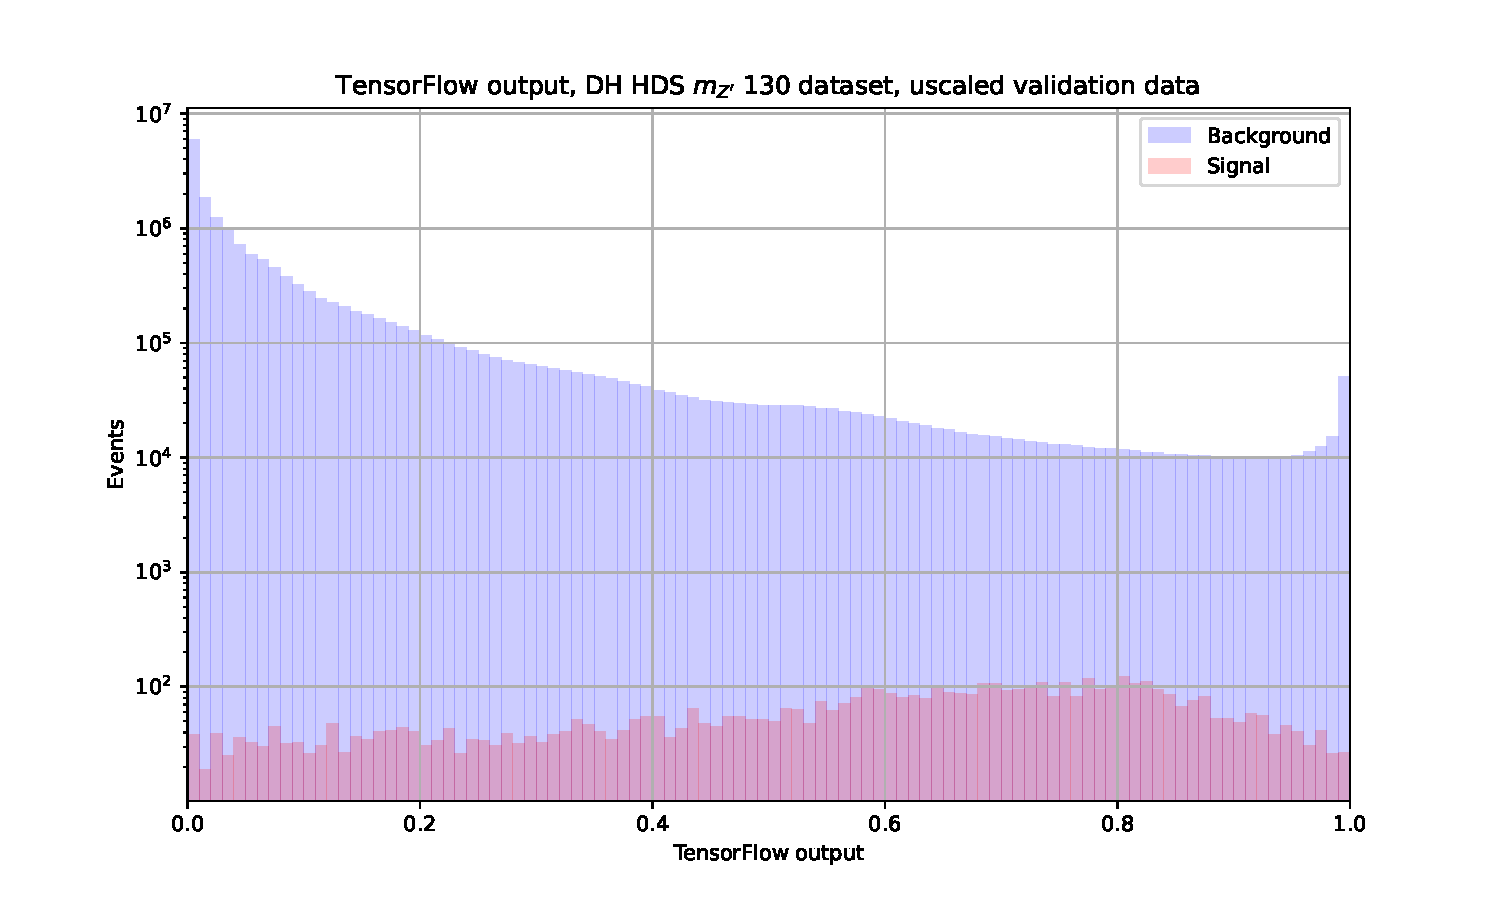
\includegraphics[width=1\textwidth]{NO_NORM/VAL_unscaled.pdf}
      \caption{No normalization}
   \end{subfigure}
   \hfill
   \begin{subfigure}[b]{0.49\textwidth}
      \centering
      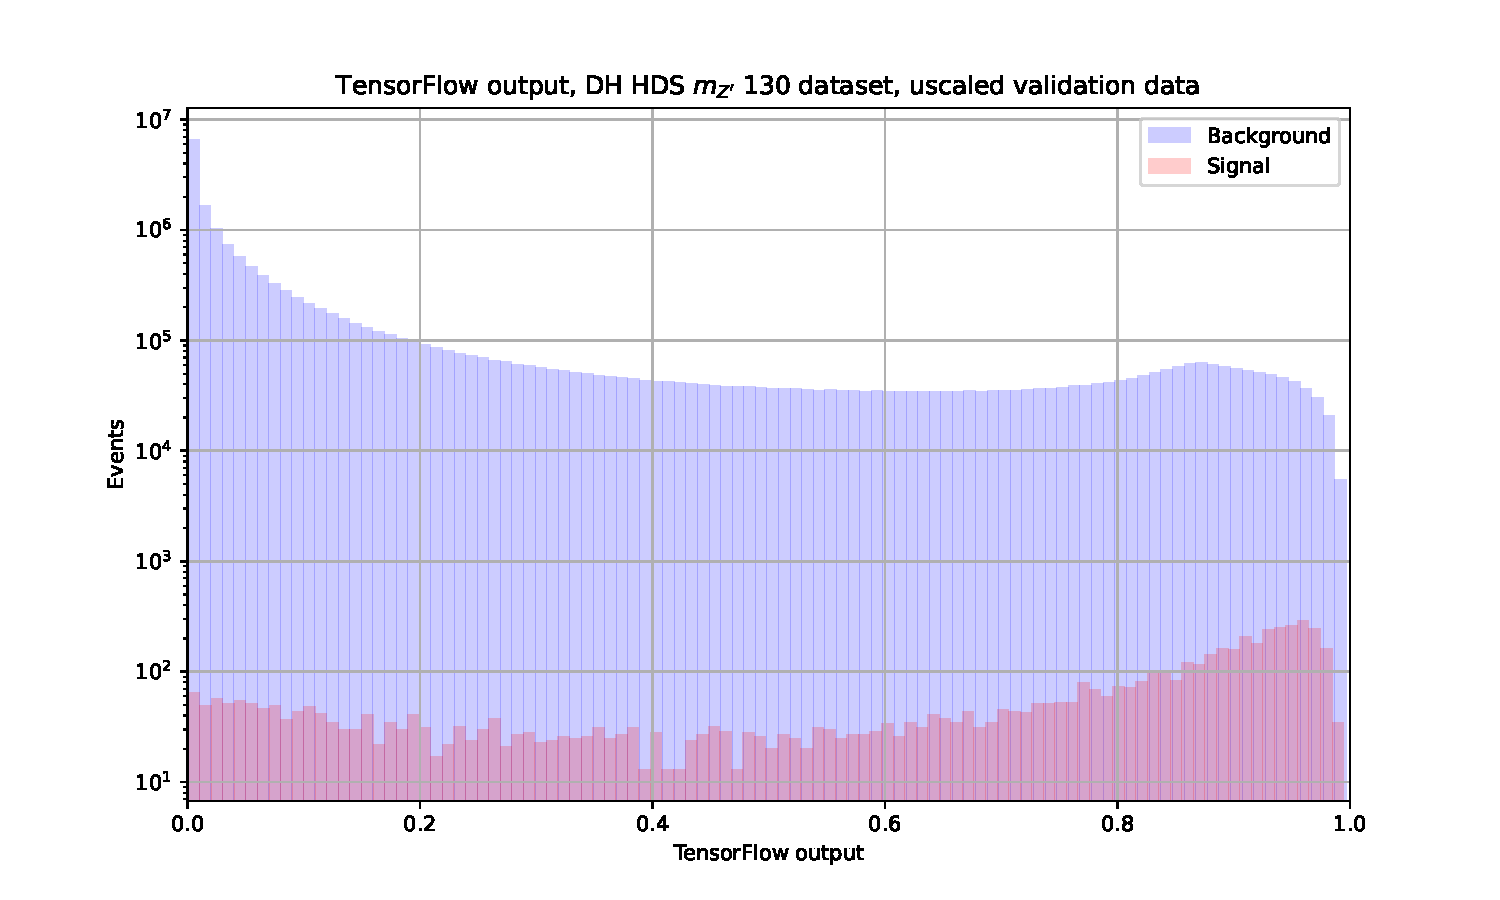
\includegraphics[width=1\textwidth]{Layer_norm/VAL_unscaled.pdf}
      \caption{Layer normalization}
   \end{subfigure}
   \hfill
	\begin{subfigure}[b]{0.49\textwidth}
      \centering
      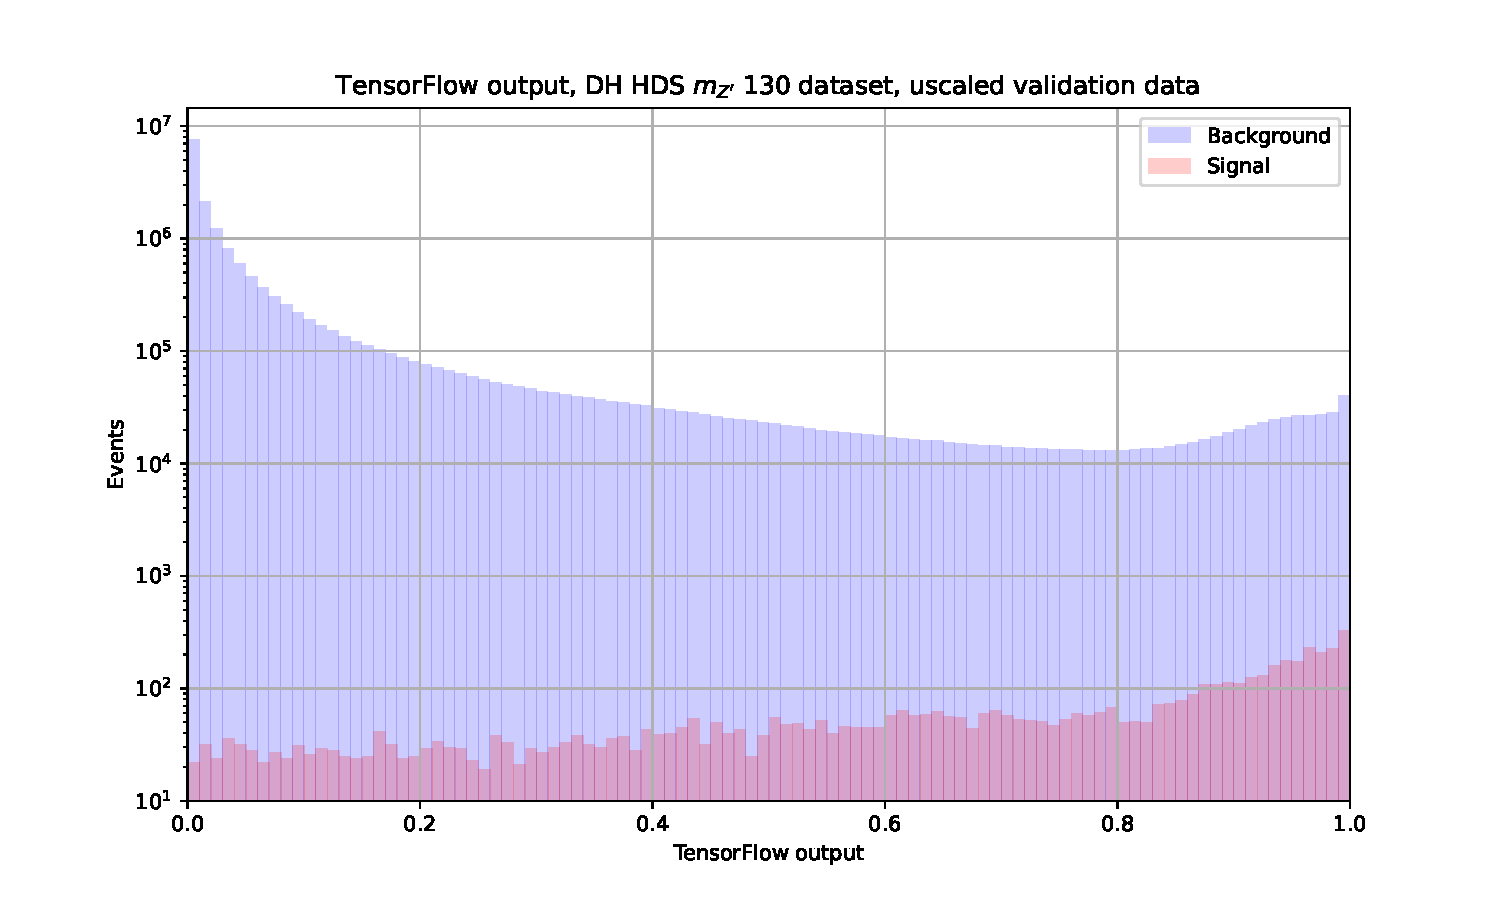
\includegraphics[width=1\textwidth]{minmax/VAL_unscaled.pdf}
      \caption{Min max scaling}
   \end{subfigure}
   \hfill\graphicspath{{../../../Plots/TESTING/NeuralNetwork/BALANCED_WEIGHTING/ONLY_BALANCE_MC_EVENTS_BKG_DOWN/DH_HDS_mZp_130/}}
   \begin{subfigure}[b]{0.49\textwidth}
      \centering
      \includegraphics[width=1\textwidth]{VAL_unscaled.pdf}
      \caption{Z-score}
   \end{subfigure}
   \hfill\graphicspath{{../../../Plots/TESTING/NeuralNetwork/NORMALIZATIONS/}}
   \begin{subfigure}[b]{0.49\textwidth}
      \centering
      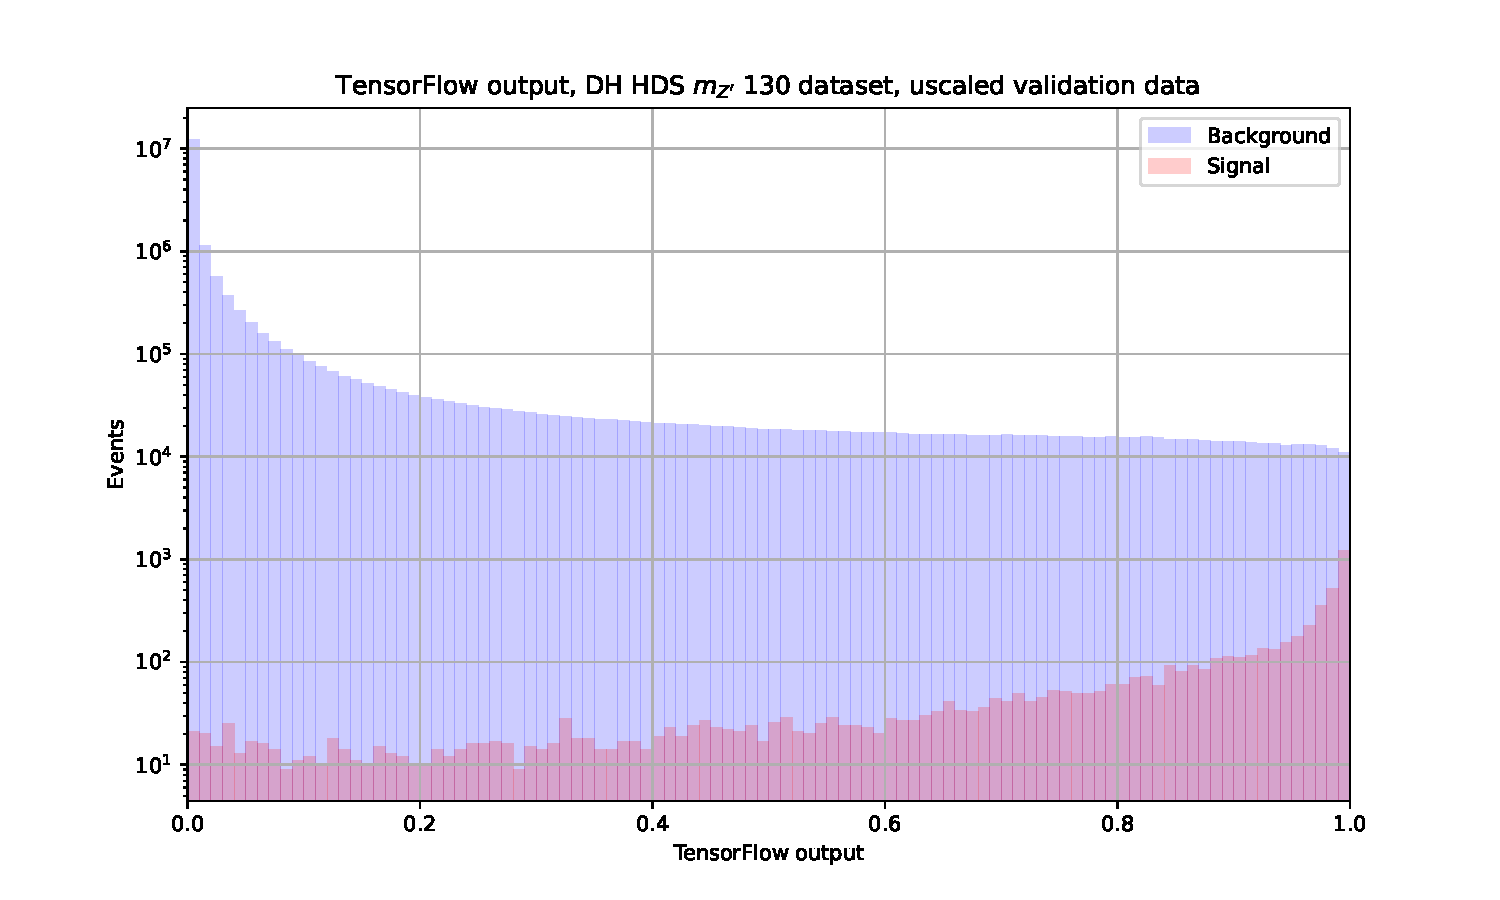
\includegraphics[width=1\textwidth]{Batch_norm/VAL_unscaled.pdf}
      \caption{Batch normalization}
   \end{subfigure}
   \caption{NN prediction when using different normalization methods. This is testing a dataset with a Z' DM model.}\label{fig:DifferentNormalizations}
\end{figure}

\graphicspath{{../../../Plots/TESTING/NeuralNetwork/BALANCED_WEIGHTING/ONLY_BALANCE_MC_EVENTS_BKG_DOWN/DH_HDS_mZp_130/}}
\begin{figure}[!ht]
	\centering
	\begin{subfigure}[b]{0.49\textwidth}
      \centering
      \includegraphics[width=1\textwidth]{VAL.pdf}
      \caption{Z-score}
   \end{subfigure}
   \hfill\graphicspath{{../../../Plots/TESTING/NeuralNetwork/NORMALIZATIONS/}}
   \begin{subfigure}[b]{0.49\textwidth}
      \centering
      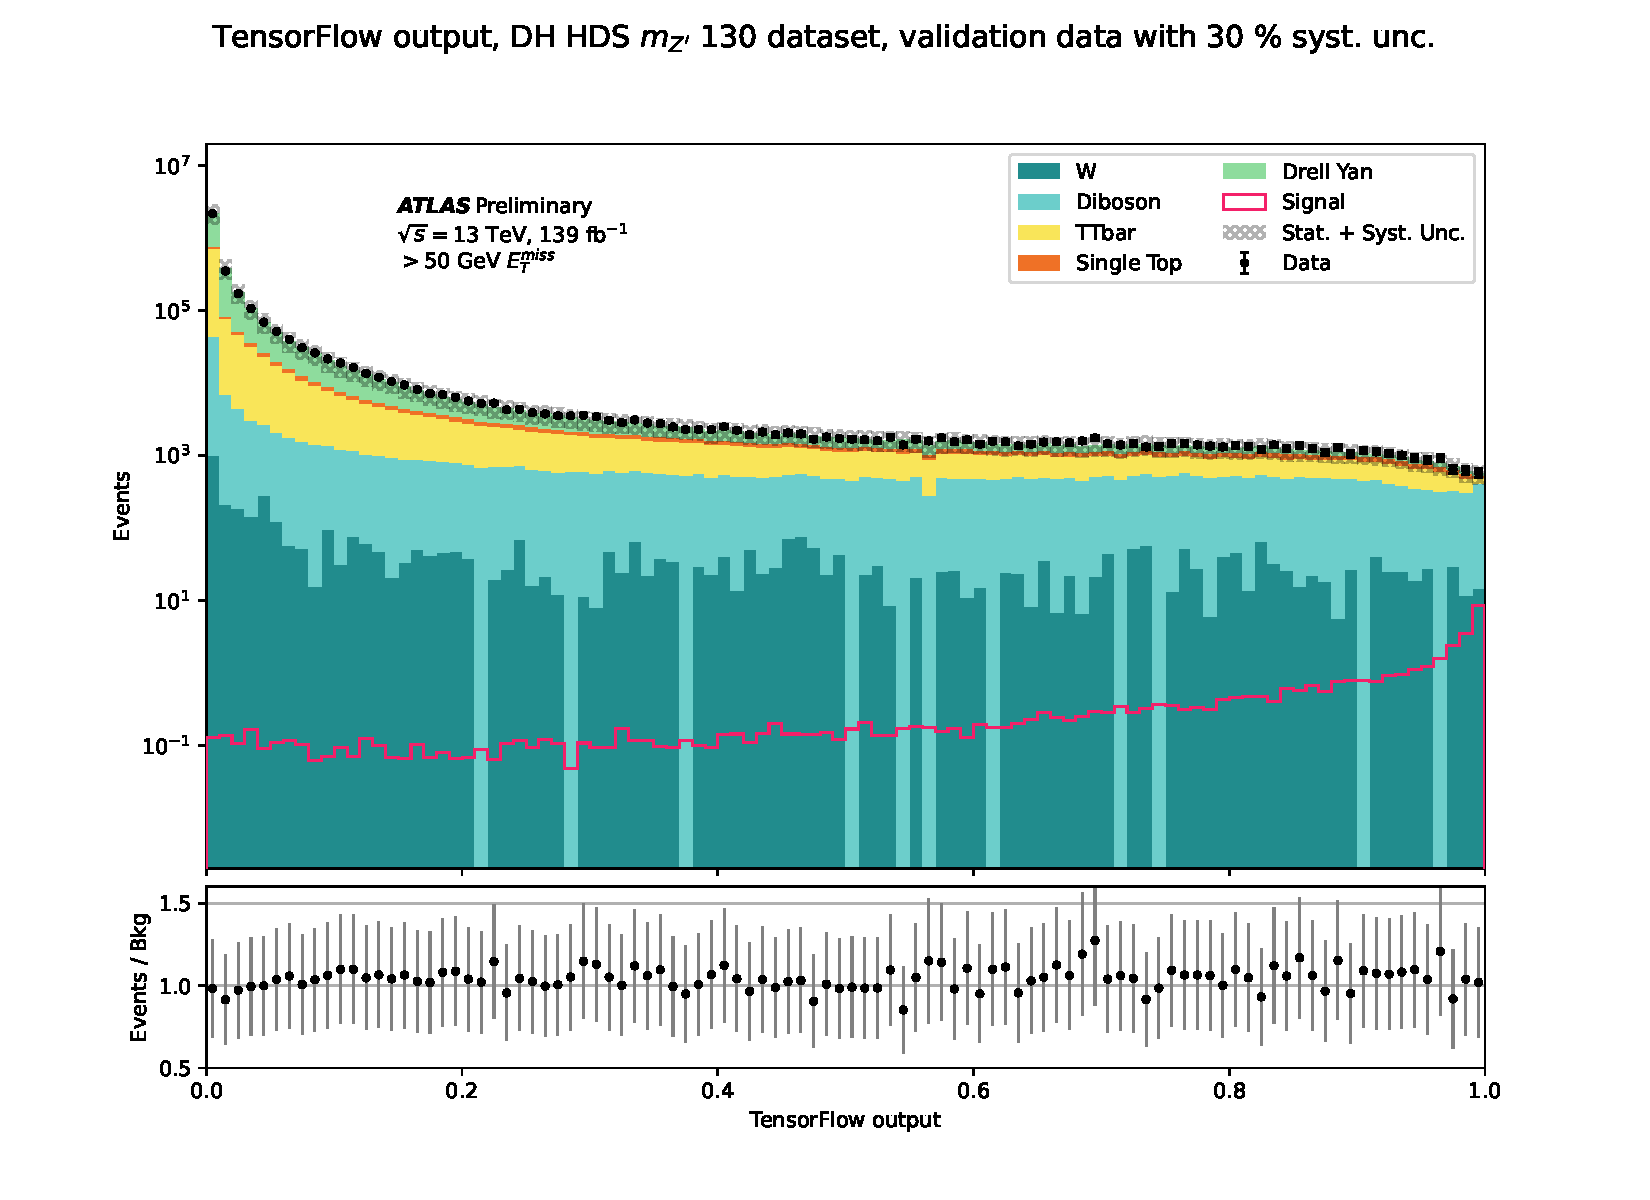
\includegraphics[width=1\textwidth]{Batch_norm/VAL.pdf}
      \caption{Batch normalization}
   \end{subfigure}
   \hfill\graphicspath{{../../../Plots/TESTING/NeuralNetwork/BALANCED_WEIGHTING/ONLY_BALANCE_MC_EVENTS_BKG_DOWN/DH_HDS_mZp_130/}}
   \begin{subfigure}[b]{0.49\textwidth}
      \centering
      \includegraphics[width=1\textwidth]{EXP_SIG.pdf}
      \caption{The expected significance of a)}
   \end{subfigure}
   \hfill\graphicspath{{../../../Plots/TESTING/NeuralNetwork/NORMALIZATIONS/}}
   \begin{subfigure}[b]{0.49\textwidth}
      \centering
      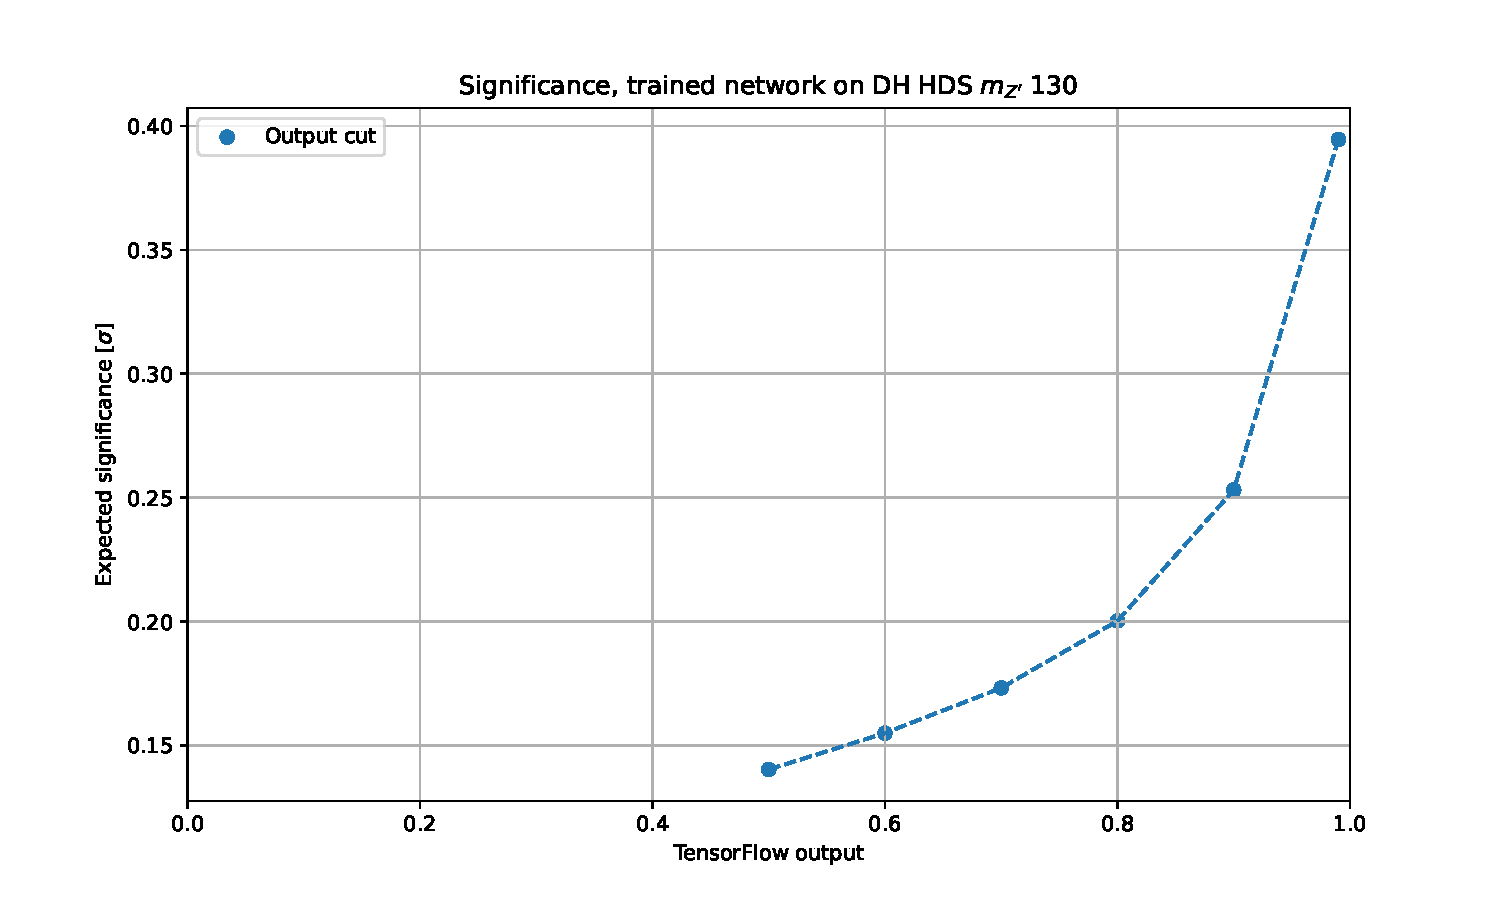
\includegraphics[width=1\textwidth]{Batch_norm/EXP_SIG.pdf}
      \caption{The expected significance of b)}
   \end{subfigure}
   \caption{Comparison of the best normalization methods. Figure a) and b) show the validation data of both cases, c) and d) show the expected significance of the validation plots when making a cut on the output. }\label{fig:BestNormie}
\end{figure}


\clearpage
\subsection{Weights}\label{sec:wgts}
\graphicspath{{../../figures/}}
The results so far (my \textit{OLD} interpretation with only three different DM theories) show that the network is completely capable of distinguishing signal from background in the unweighted training, however if we were to scale the predictions (the networks output) with the weights (sample weights * luminosity / sum of weights) we would see that the signal is hidden underneath the background. Both validation plots are shown in Figure \ref{fig:OLD_FULL_DM_VAL}. If we train the network using the weights of the MC samples we see that the network still gets the same accuracy, and an even lower loss function score. But the AUC becomes exactly 0.5. When looking at the ROC curve and validation plots (plots showing how well the network sorts signal from background) we see that everything "is messed up" the ROC is 0.5, and there is only \textbf{one} background bin. When printing how many signal events the weighted network predicted it is easy to understand why, it is because it says there is not a single dark matter event. Which I first interpreted as being in agreement with Figure \ref{fig:OLD_W_FULL_DM_VAL}.\\
\begin{figure}[!ht]
	\centering
	\begin{subfigure}[b]{0.8\textwidth}
        \centering
        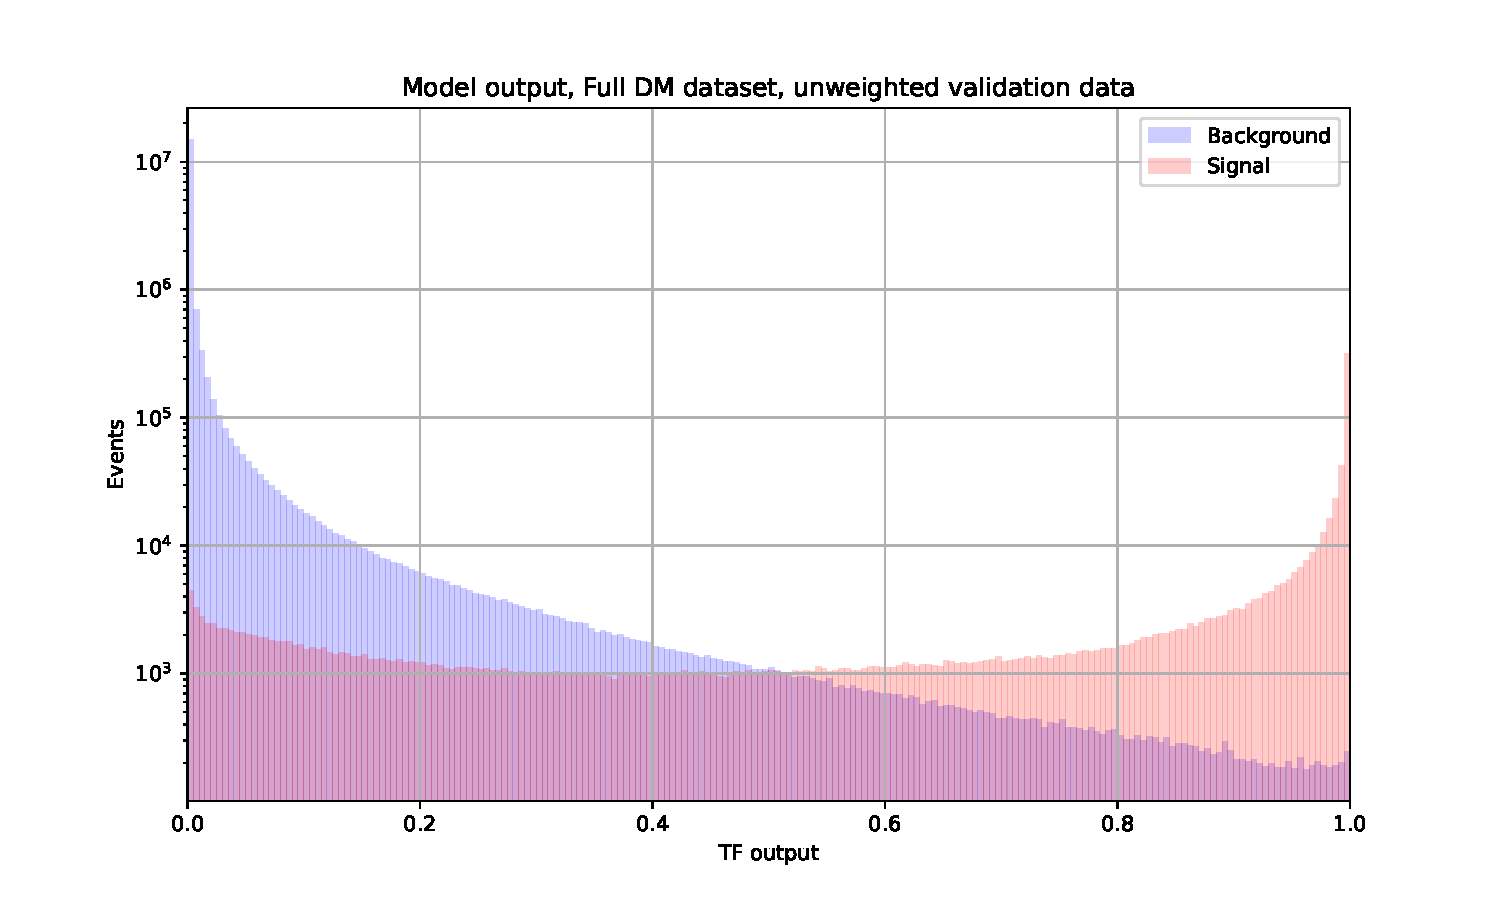
\includegraphics[width=1\textwidth]{OLD_DM_FULL_VAL_UNW.pdf}
        \caption{Unscaled validation plot.}\label{fig:OLD_UNW_FULL_DM_VAL}
     \end{subfigure}
     \hfill
     \begin{subfigure}[b]{0.8\textwidth}
        \centering
        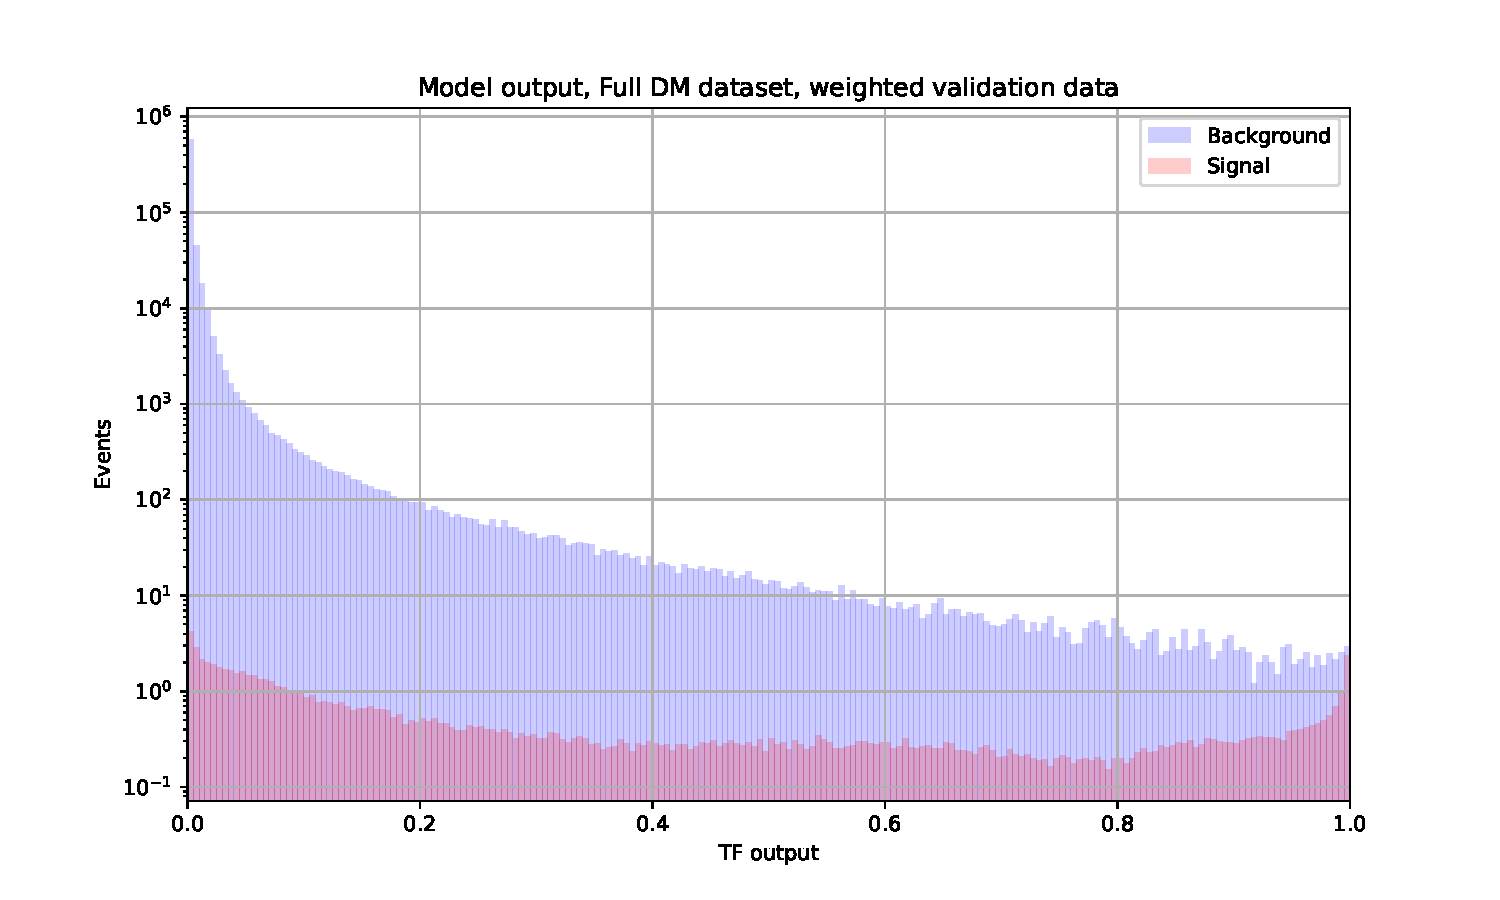
\includegraphics[width=1\textwidth]{OLD_DM_FULL_VAL_W.pdf}
        \caption{Scaled validation plot using MC weights.}\label{fig:OLD_W_FULL_DM_VAL}
     \end{subfigure}
	\caption{Validation plot of uwweighted network on the first version of the FULL DM dataset.}\label{fig:OLD_FULL_DM_VAL}
\end{figure}
\\\todo{The italics were my thoughts at the time}\textit{From my understanding it is preferable to train the network with weights, because then we can use it to predict data events, which have physical significance compared to MC events. This will be specially useful in my head when we predict how many dark matter events there are using real data, as this cannot be "scaled up" at a later point.}\\
\\\textit{As to which weights one shall use I am unsure, I like the physical weights for the reason above. But I know that for uneven datasets one could "weight down" the background events such that it "looks to be a 50-50 ratio" between background in signal. This sounds like making a bias in my head, and I would not know how to interpret the network predictions (if it predicts samples or events), but this appears to be a "standard" technique used in data science.}\\
\\T\textit{o check whether the network is working as intended I will now try to sort out "Diboson" events from other SM backgrounds, since we know this is real. If it works as intended I am unsure as to where to go next.} One thing worth noting is that the weights for the dark matter models being used may not necessarily be correct, as we don't have any empirical proof for the variables being used when calculating the weights (i.e. the cross section). \\
\\It seems that my interpretation was wrong, the weighted network for the Diboson search also predicted "0 Diboson events" (meaning my interpretation of the network predicting number of events is wrong), something we can empirically say is wrong (i.e. literally every figure of the kinematic variables). The scaled validation plot of the unweighted signal still "shows" that the network struggles a bit to see the difference between signal and background, overlapping almost all the way to 0.8. However it is still capable of sorting it out. Now I will try the "data analysts" way to weight the samples. That means weighting all background samples by $\frac{N_{sig}}{N_{bkg}}$, as is a common practice of weighting unbalanced datasets in data analysis.\\
\\The new weighting works! This is the method that will be used in the further studies using NNs. The \textit{Validation plots} showing the results of the network when trying to sort out the "Diboson" channel from the other are shown in Figure \ref{fig:DibosonVAL} and the ROC scores in Figure \ref{fig:DibosonROC}. A table showing how unbalanced the data is is showcased in Table \ref{tab:UnbalancedDibosonTraining}.\\
\begin{figure}[!ht]
	\centering
	\begin{subfigure}[b]{0.8\textwidth}
        \centering
        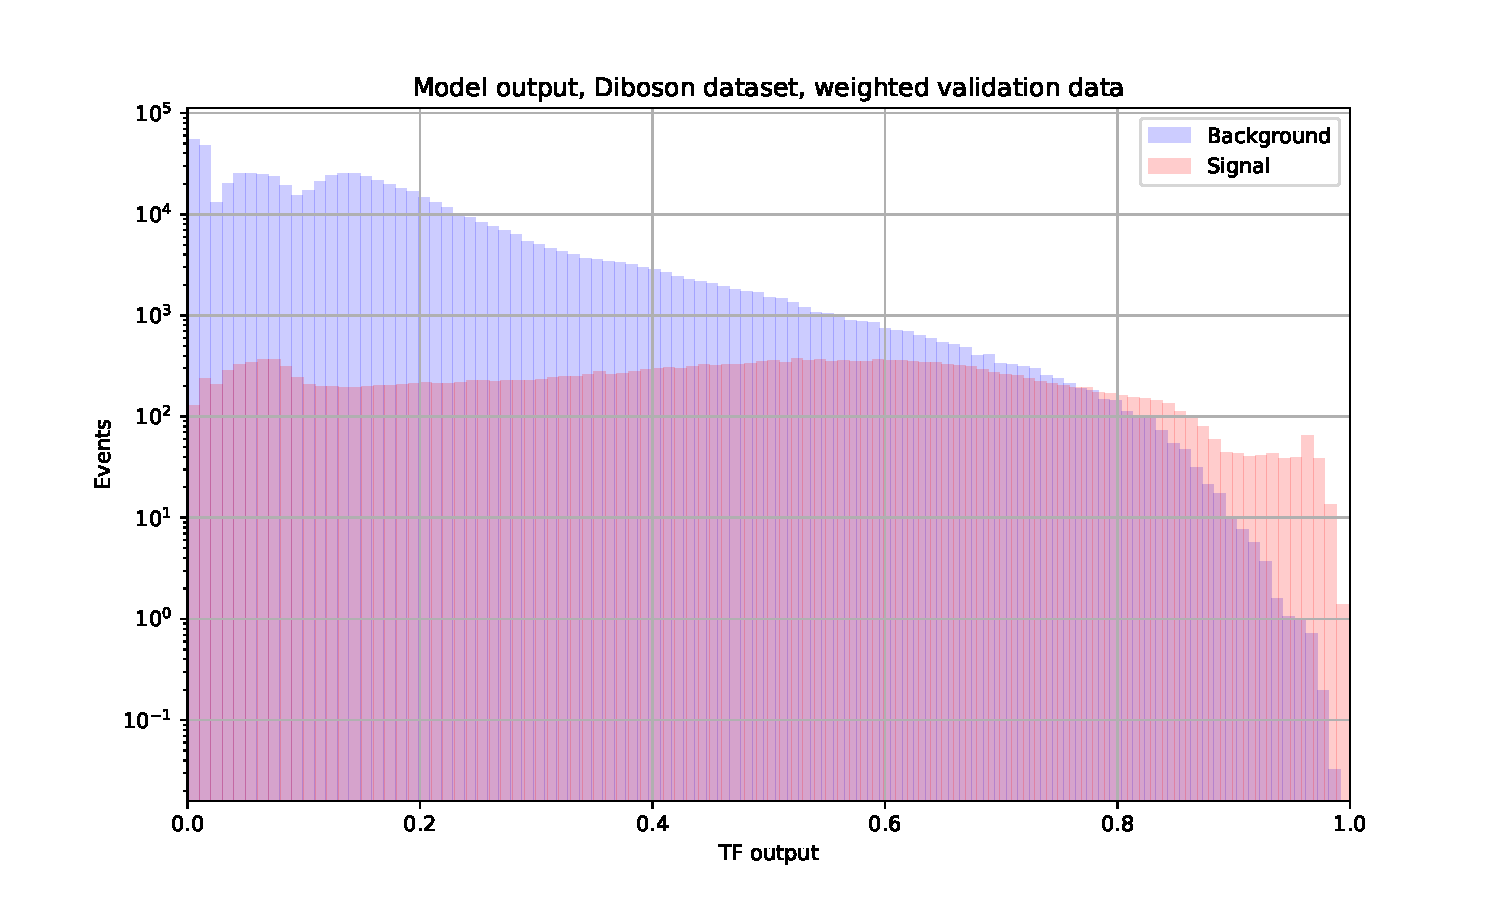
\includegraphics[width=1\textwidth]{VAL_uw.pdf}
        \caption{Validation plot for the unweighted training.}\label{fig:DibosonVALUW}
     \end{subfigure}
     \hfill
     \begin{subfigure}[b]{0.8\textwidth}
        \centering
        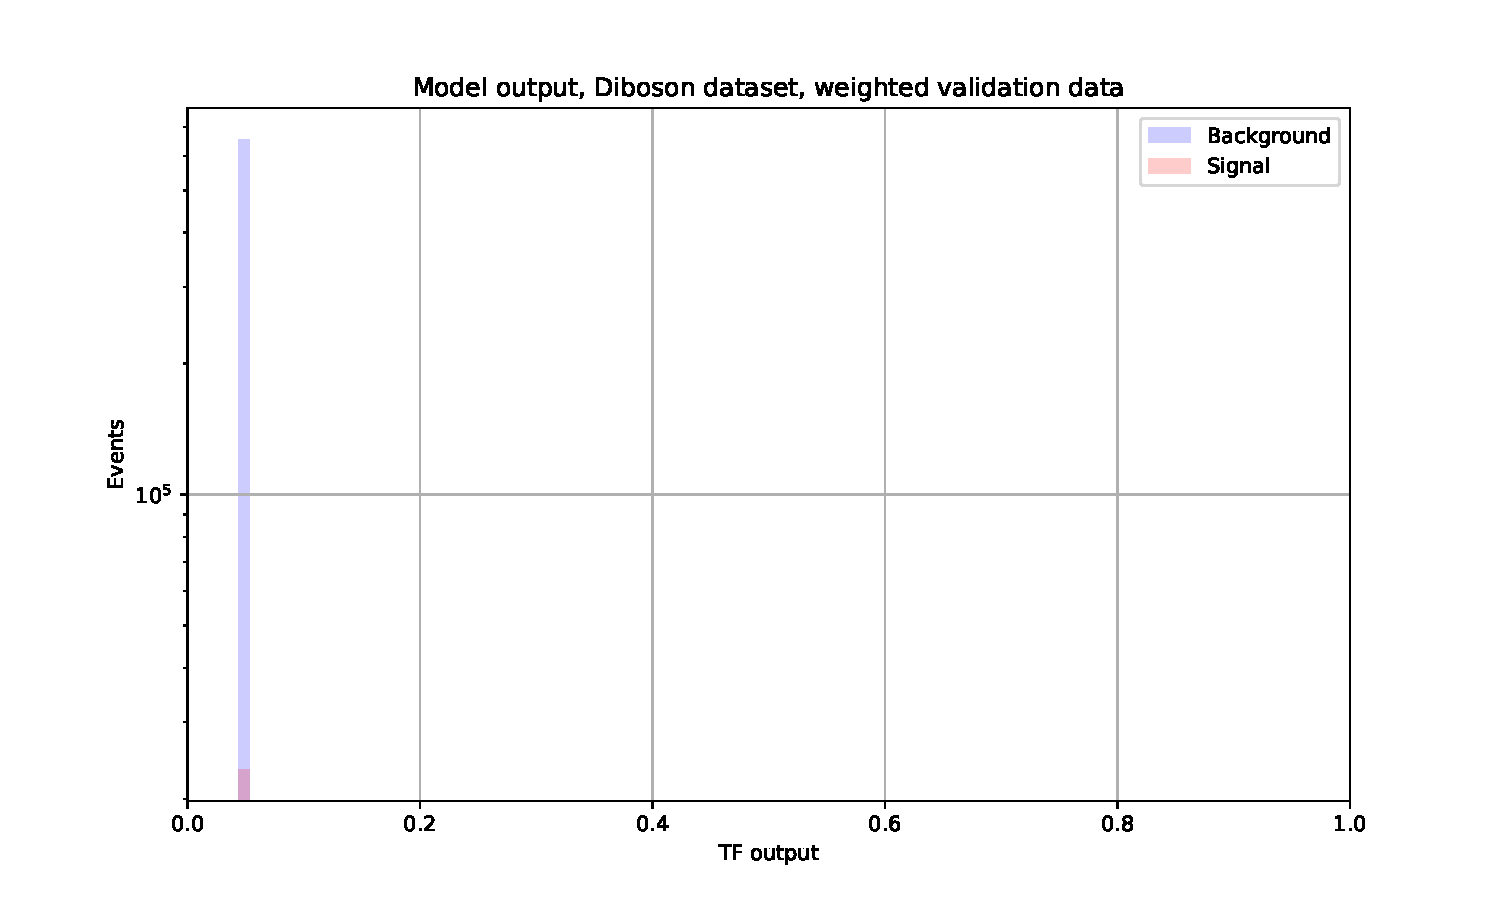
\includegraphics[width=1\textwidth]{VAL_mc.pdf}
        \caption{Validation plot for the weighted training using MC weights.}\label{fig:DibosonVALMC}
     \end{subfigure}
     \begin{subfigure}[b]{0.8\textwidth}
        \centering
        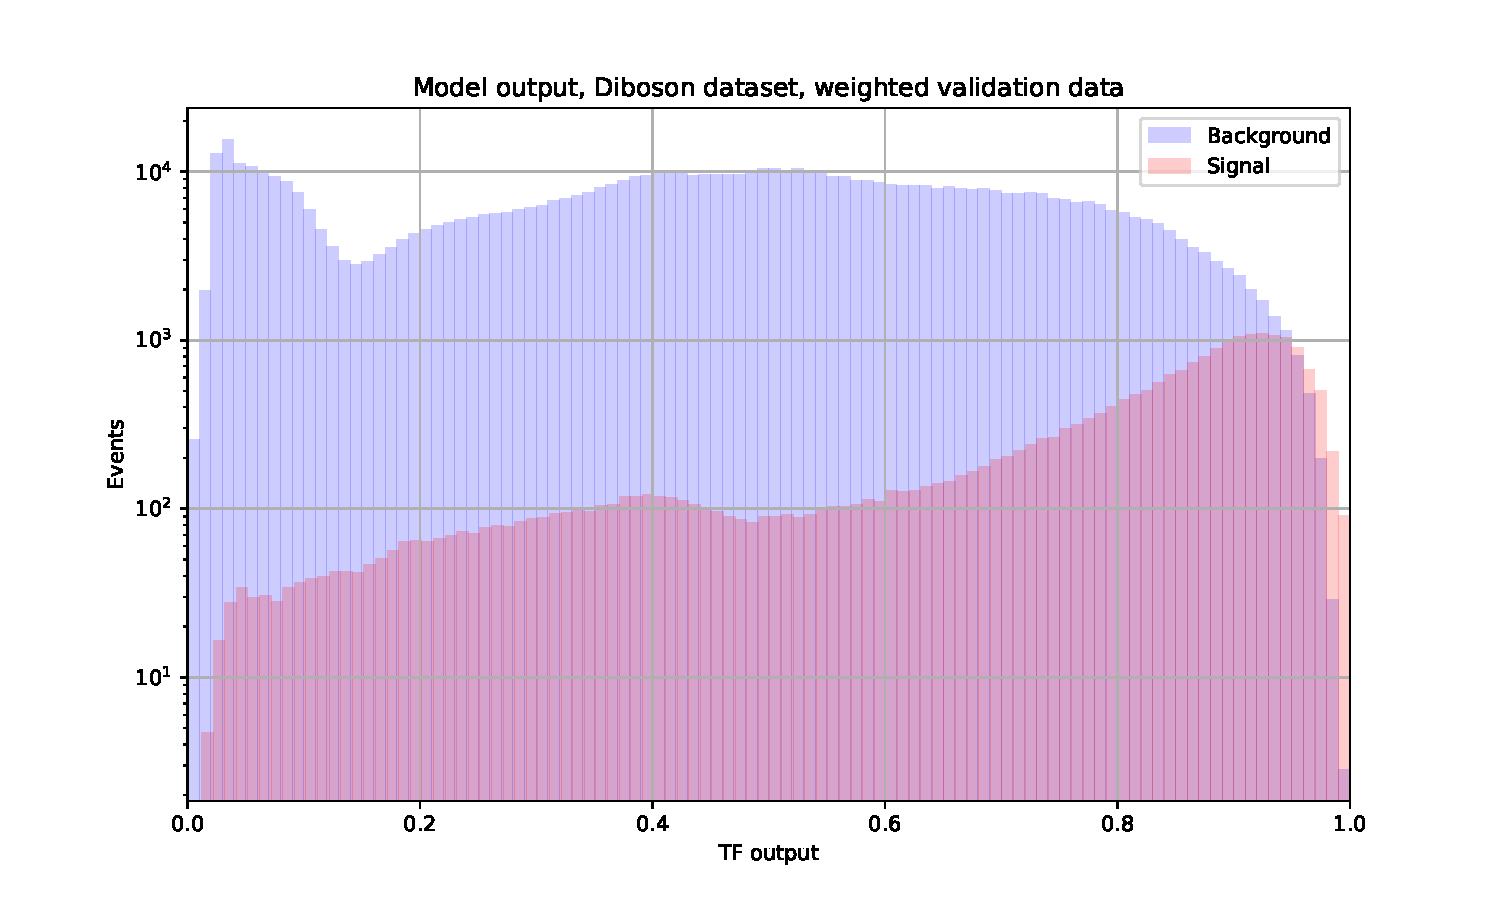
\includegraphics[width=1\textwidth]{VAL_w.pdf}
        \caption{Validation plot for the weighted training using $\frac{N_{sig}}{N_{bkg}}$ as weights on the background.}\label{fig:DibosonVALW}
     \end{subfigure}
	\caption{Result of the different network training weighting.}\label{fig:DibosonVAL}
\end{figure}
\begin{figure}[!ht]
	\centering
	\begin{subfigure}[b]{0.49\textwidth}
        \centering
        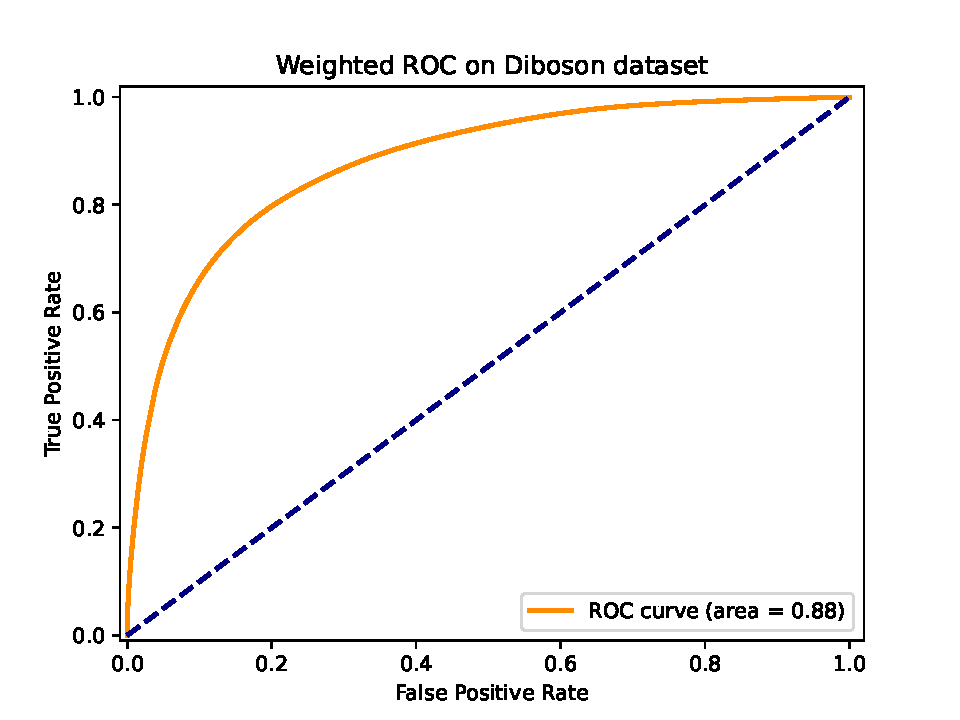
\includegraphics[width=1\textwidth]{ROC_uw.pdf}
        \caption{ROC score for the unweighted training.}\label{fig:DibosonROCUW}
     \end{subfigure}
     \hfill
     \begin{subfigure}[b]{0.49\textwidth}
        \centering
        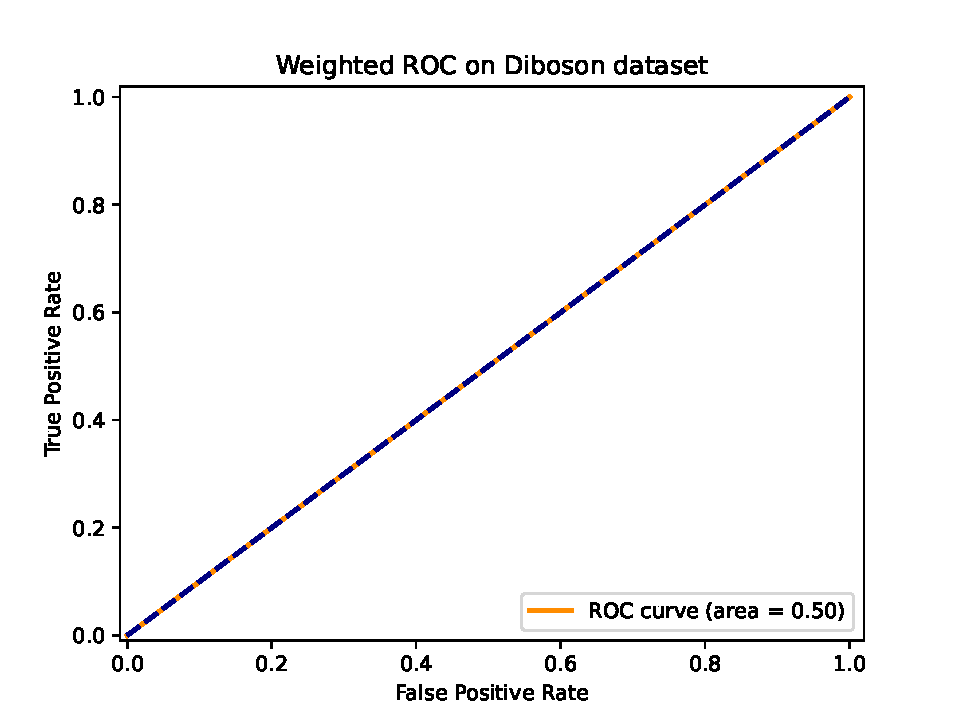
\includegraphics[width=1\textwidth]{ROC_mc.pdf}
        \caption{ROC score for the weighted training using MC weights.}\label{fig:DibosonROCMC}
     \end{subfigure}
     \begin{subfigure}[b]{0.49\textwidth}
        \centering
        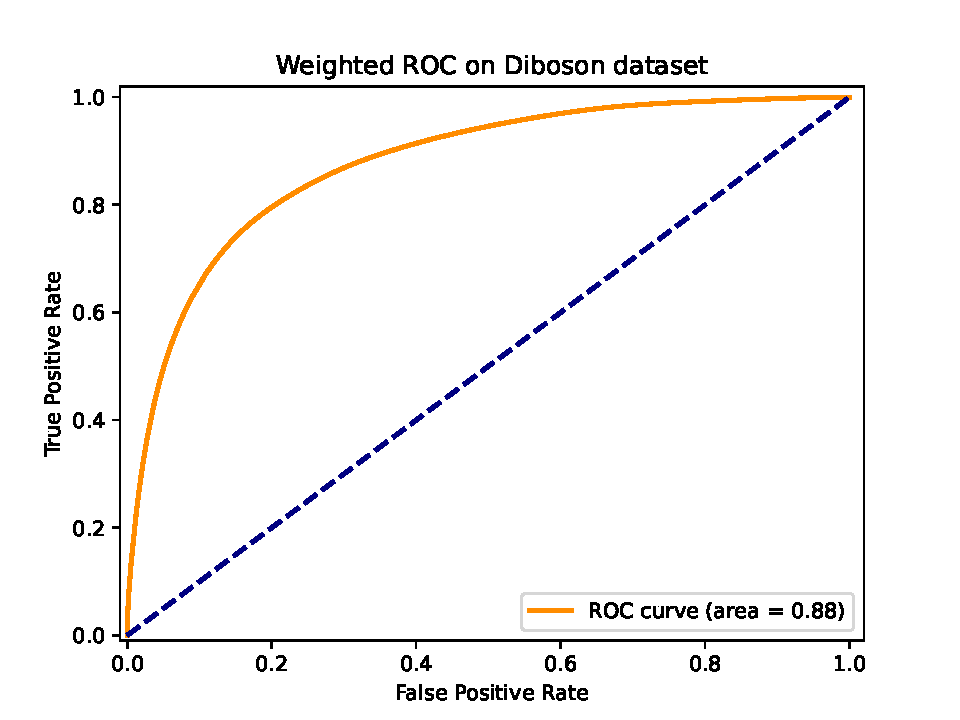
\includegraphics[width=1\textwidth]{ROC_w.pdf}
        \caption{ROC score for the weighted training using $\frac{N_{sig}}{N_{bkg}}$ as weights on the background.}\label{fig:DibosonROCW}
     \end{subfigure}
	\caption{Result of the different network training weighting.}\label{fig:DibosonROC}
\end{figure}
\begin{table}[!h]
    \centering
    \begin{tabular}{l|r|r|r}\midrule\midrule
                    & Number of events & Sum of weights & Events $\times$ SOW [$10^{11}$]\\\midrule
         Signal     & 8,813,716        & 93,304.9       & 8.2\\
         Background & 61,201,010       & 2,621,498.9    & 1,604.4 \\ \midrule\midrule
    \end{tabular}
    \caption[Unbalanced Diboson training dataset]{Table Showcasing how uneven the training dataset is between signal and background. This is on the Diboson dataset which incorporates all the SM MC samples}
    \label{tab:UnbalancedDibosonTraining}
\end{table}

\clearpage
\subsection{Balanced weights}\label{sec:Balanced_wgts}
Even if the weighting method previously described helps the network to give reasonable results. It most likely won't distinguish the importance between signal events that have high resonance and those that do not. 
As an example, if we look at the Z' DH model in the HDS and compare how the network classifies a model with a $m_{Z'}$ of 130 GeV to one with a $m_{Z'}$ of 1500 GeV we might get an idea of how the network classifies things.
We can see how the network predicts wether an event is signal or background using validation plots, this is seen in \ref{fig:PurelyBalanced_DH_HDS}.
\graphicspath{{../../../Plots/TESTING/NeuralNetwork/BALANCED_WEIGHTING/ONLY_BALANCE_MC_EVENTS_BKG_DOWN/}}
\begin{figure}[!ht]
	\centering
	\begin{subfigure}[b]{0.49\textwidth}
        \centering
        \includegraphics[width=1\textwidth]{DH_HDS_mZp_130/VAL_unscaled.pdf}
        \caption{NN prediction of DH HDS $m_{Z'}$ = 130 GeV}\label{fig:PurelyBalanced_DH_HDS_130}
     \end{subfigure}
     \hfill
     \begin{subfigure}[b]{0.49\textwidth}
        \centering
        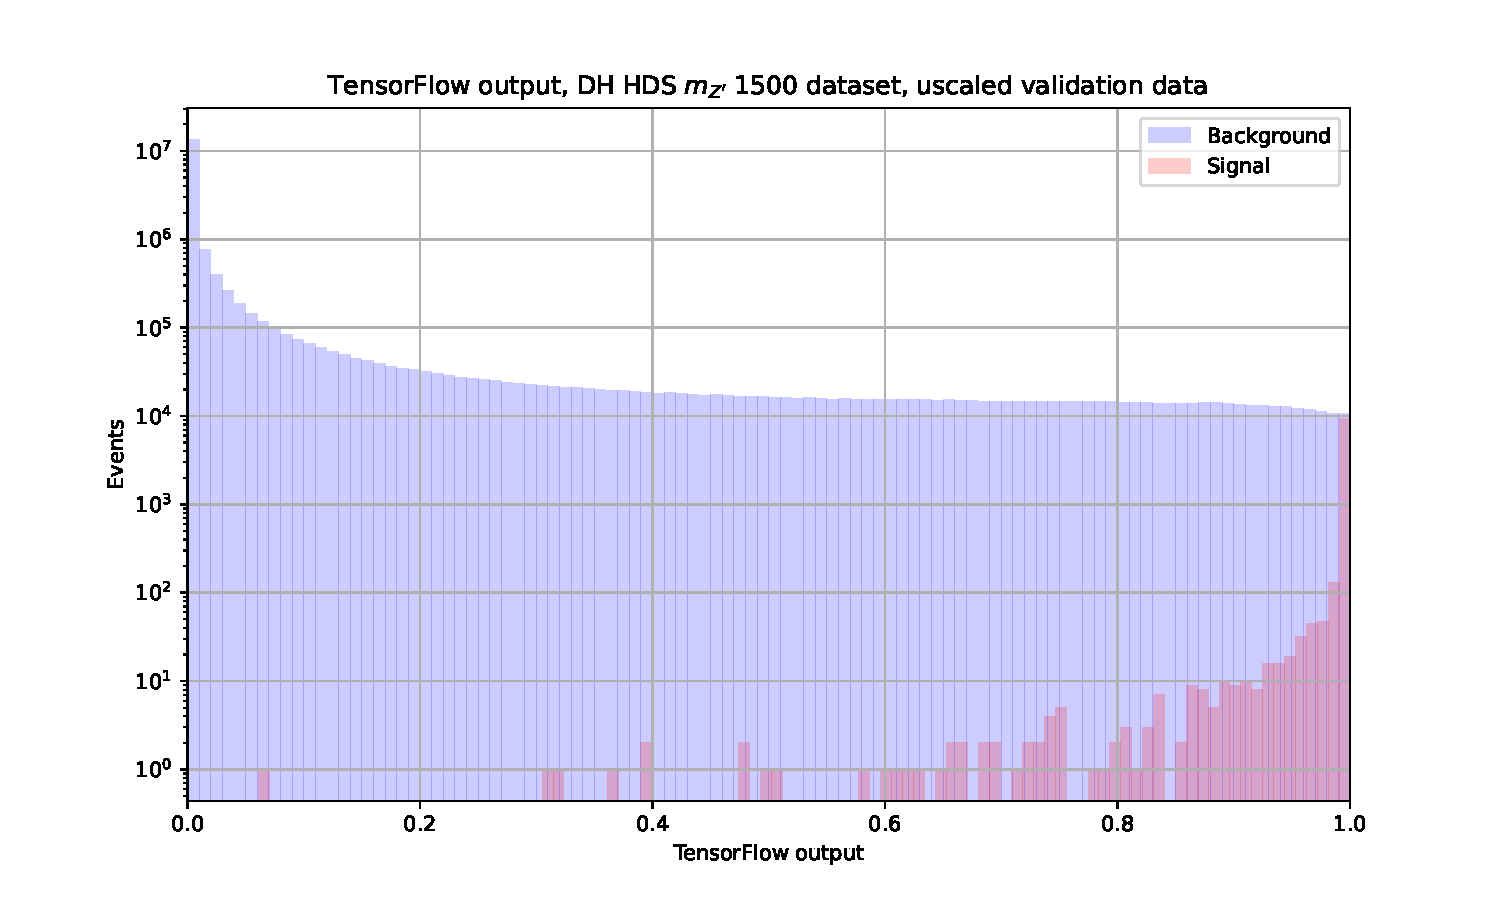
\includegraphics[width=1\textwidth]{DH_HDS_mZp_1500/VAL_unscaled.pdf}
        \caption{NN prediction of DH HDS $m_{Z'}$ = 1500 GeV}\label{fig:PurelyBalanced_DH_HDS_1500}
     \end{subfigure}
     \caption{NN comparison of trained models in FULL Z' dataset}\label{fig:PurelyBalanced_DH_HDS}
\end{figure}
\\The result purely demonstrate the raw network output, meaning that the validation dataset has not been scaled up using MC weights (i.e. model cross section) or luminosity.\\
\\We can see the network is better at classifying the events from the model with $m{Z'}$ = 1500 GeV than the other, even if this model has a much lower cross section, as seen in the correctly scaled plots below.
\begin{figure}[!ht]
	\centering
	\begin{subfigure}[b]{0.49\textwidth}
        \centering
        \includegraphics[width=1\textwidth]{DH_HDS_mZp_130/VAL.pdf}
        \caption{NN prediction of DH HDS $m_{Z'}$ = 130 GeV}
     \end{subfigure}
     \hfill
     \begin{subfigure}[b]{0.49\textwidth}
        \centering
        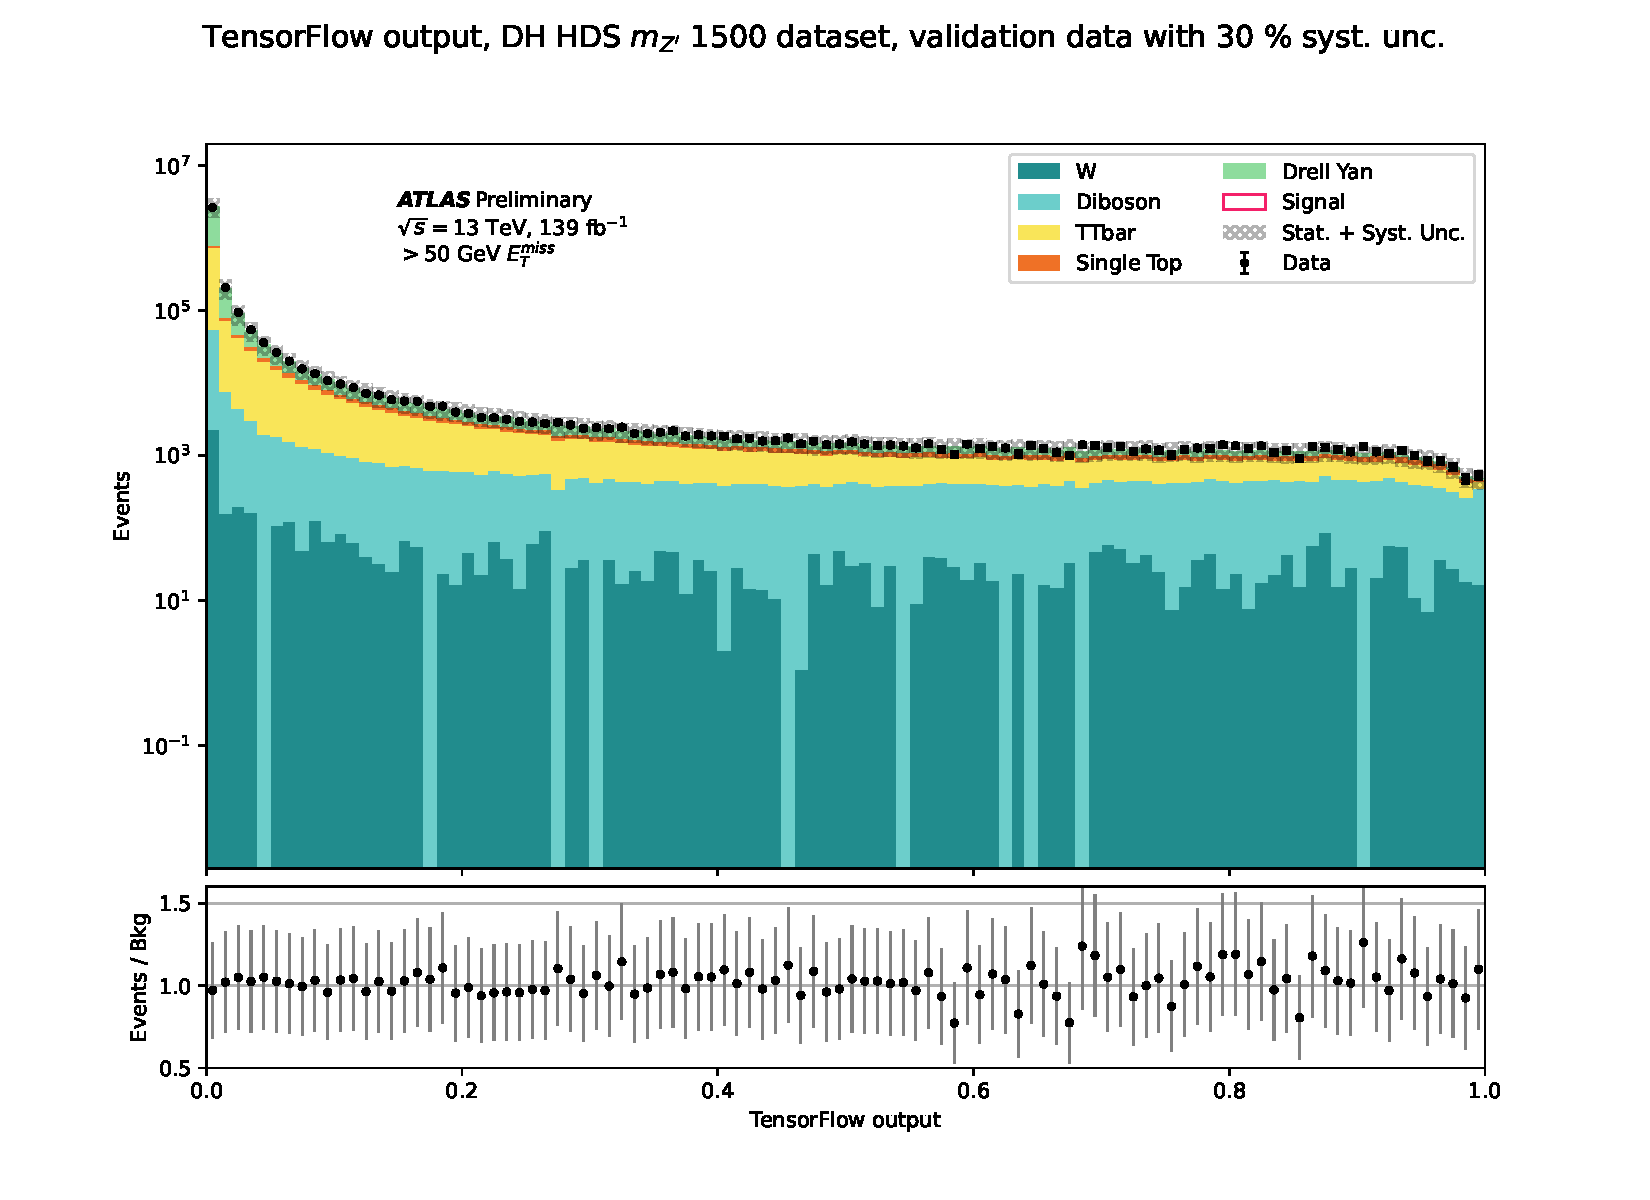
\includegraphics[width=1\textwidth]{DH_HDS_mZp_1500/VAL.pdf}
        \caption{NN prediction of DH HDS $m_{Z'}$ = 1500 GeV}
     \end{subfigure}
     \caption{Correctly scaled plots.}\label{fig:SCALED_PurelyBalanced_DH_HDS}
\end{figure}
\\As we can clearly see, the better predicted model by the network does not even have one event when scaled up correctly. Therefore it is desirable to both take into account the data imbalance between the signal and background as well as the MC weights when training a network. To do this using TensorFlow we could make use of two parameters when training the network: \verb|class_weight| and \verb|sample_weight|.
\\\\\verb|class_weight| works as a dictionary that weights events that are keys on the dictionary. For our purposes we can make a dictionary where we weight signal and background events differently, this is the same type of scaling that was done in the previous section. 
\verb|sample_weight| takes in individual weights for every single event that goes into the netwrok, meaning that it is crucial that we know that the desired weight matches the desired event. Ideally we would use both weighting methods, \verb|class_weight| to balance the signal to background ratio and \verb|sample_weight| with the MC weights. 
However there is a bug in TensorFlow (up to version \verb|GPU 2.7.1|) that makes it so the program doesn't run when using both parameters. This is not a big problem though, as when looking at the source code one can see that what TensorFlow does with both weights is multiply them togheter. Thus we could try to make use of this "balaned weighting" method to see if the network learns the different models better.\\
\\We can see in Table \ref{tab:MC_imbalance} how uneven the data (FULL Z') is. To balance the data we have four options. We can either \textit{weigh up the signal} events by the ratio of background over signal. Or \textit{weigh down the bacgkround} with the ratio of signal over background. However this ratio might differ a lot when using the MC raw event ratio or the SOW events ratio. I have tested all four possibilities and these can be see below.\\
\begin{table}[!h]
   \centering
   \begin{tabular}{l|c|c}\midrule\midrule
                        & Actual events   & MC events \\\midrule
         Background     & 2,715,280.4     & 69,664,290  \\
         Signal         & 388.4           & 2,991,598   \\\midrule\midrule
   \end{tabular}
   \caption[Imbalance raw events and SOW]{Table showcasing the data imbalance between background and signal in both raw MC events and actual events. By actual events it is meant weighted events. This is for the training dataset on the FULL Z' dataset.}
   \label{tab:MC_imbalance}
\end{table}
\graphicspath{{../../../Plots/TESTING/NeuralNetwork/BALANCED_WEIGHTING/MC_WGT_SIG_UP/}}
\begin{figure}[!ht]
	\centering
	\begin{subfigure}[b]{0.49\textwidth}
        \centering
        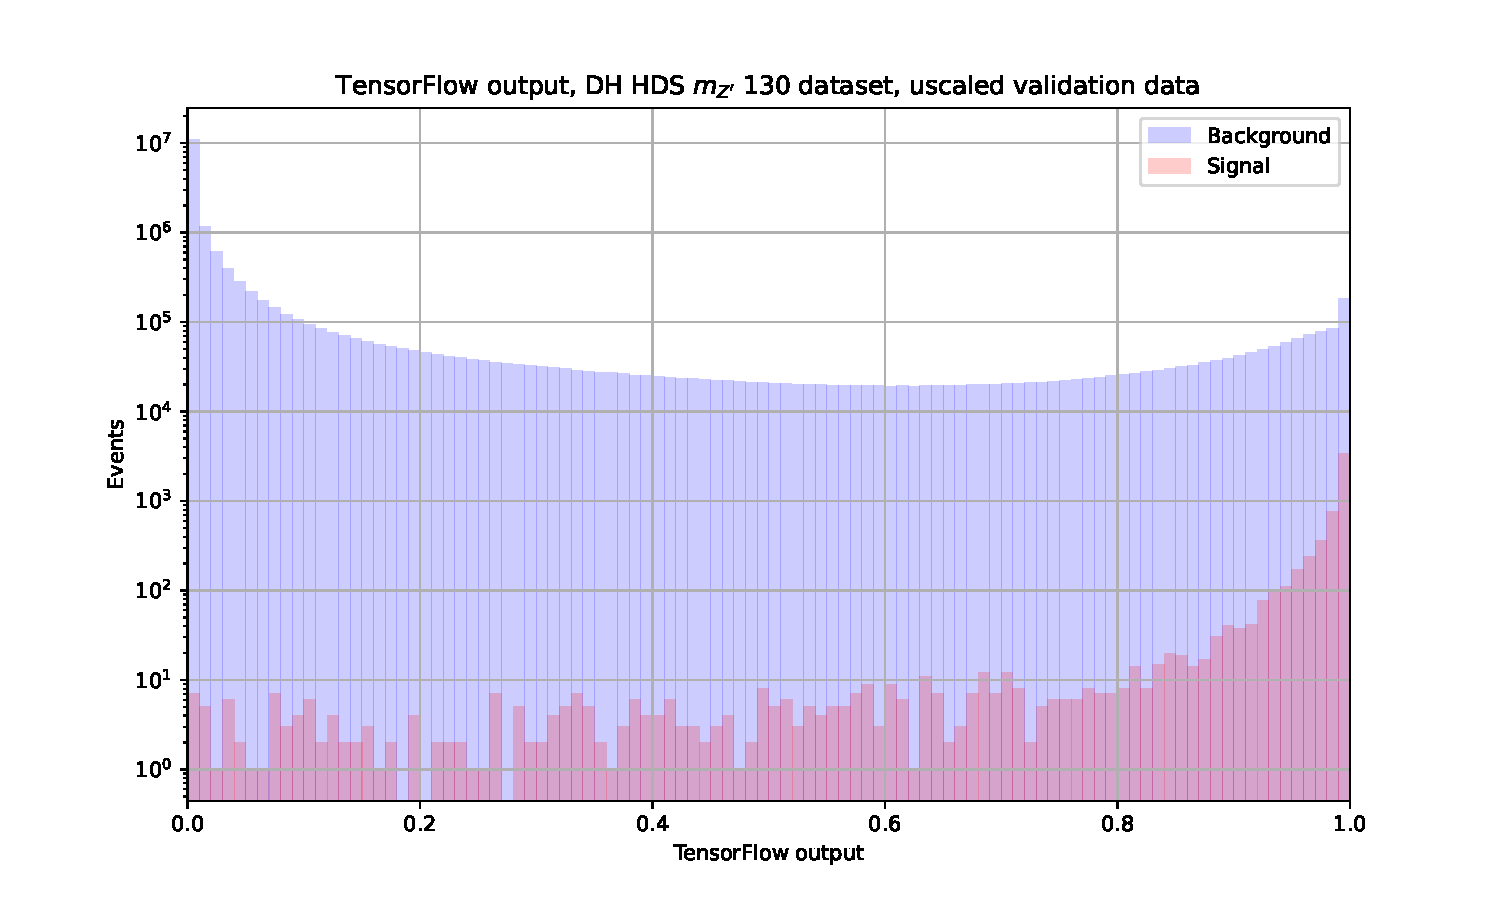
\includegraphics[width=1\textwidth]{DH_HDS_mZp_130/VAL_unscaled.pdf}
        \caption{NN prediction of DH HDS $m_{Z'}$ = 130 GeV}\label{fig:MC_WGT_SIG_DH_HDS_130}
     \end{subfigure}
     \hfill
     \begin{subfigure}[b]{0.49\textwidth}
        \centering
        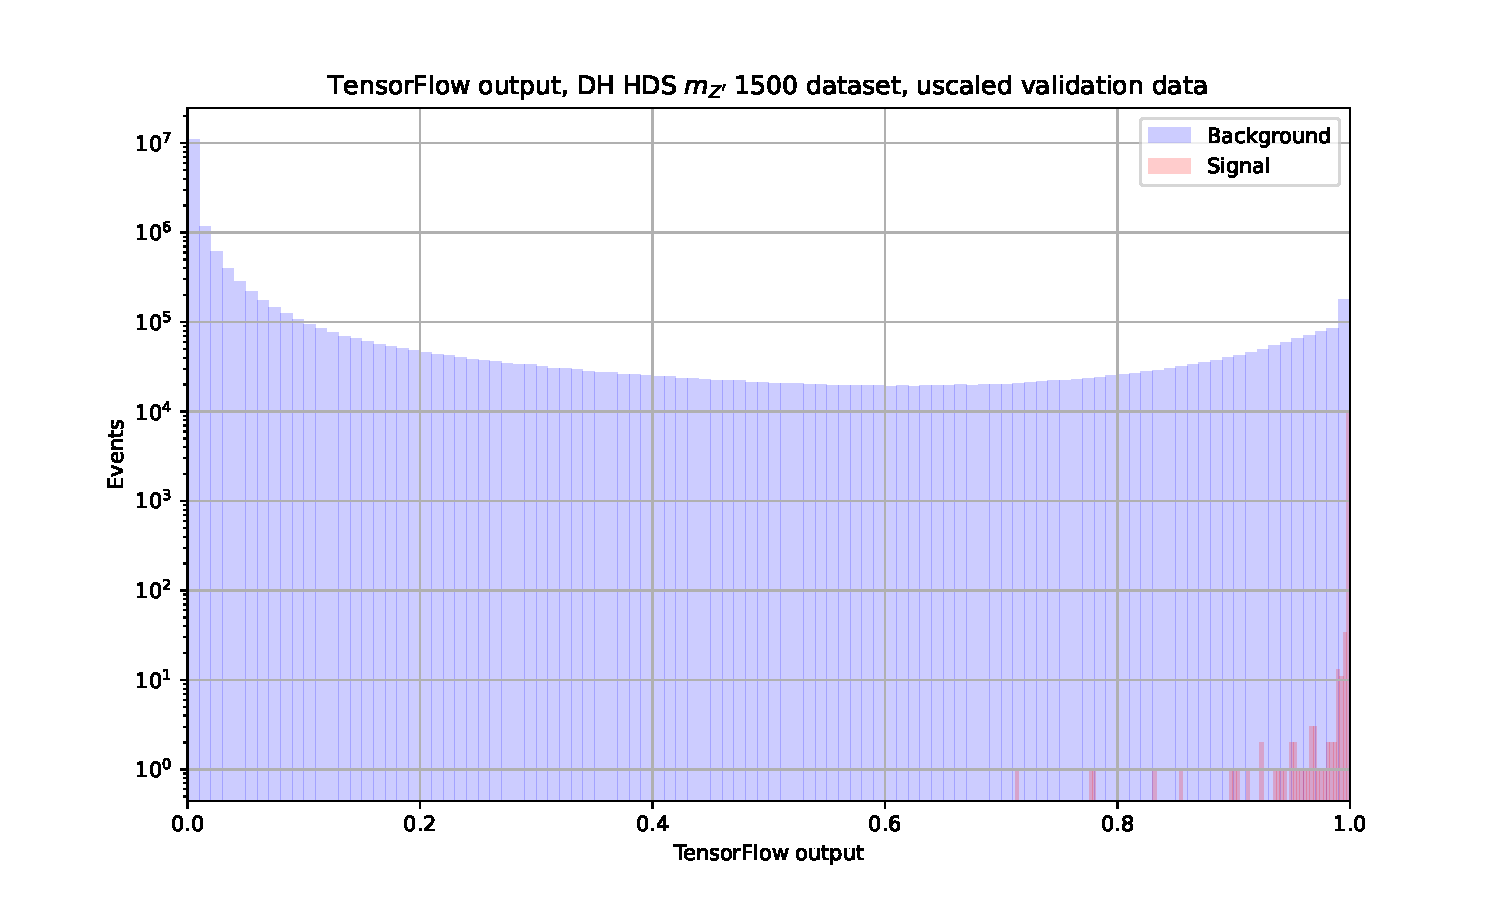
\includegraphics[width=1\textwidth]{DH_HDS_mZp_1500/VAL_unscaled.pdf}
        \caption{NN prediction of DH HDS $m_{Z'}$ = 1500 GeV}\label{fig:MC_WGT_SIG_DH_HDS_1500}
     \end{subfigure}
     \caption{NN prediction when weighting the signal with the SOW ratio.}\label{fig:MC_WGT_SIG_DH_HDS}
\end{figure}
\graphicspath{{../../../Plots/TESTING/NeuralNetwork/BALANCED_WEIGHTING/MC_EVENTS_SIG_UP/}}
\begin{figure}[!ht]
	\centering
	\begin{subfigure}[b]{0.49\textwidth}
        \centering
        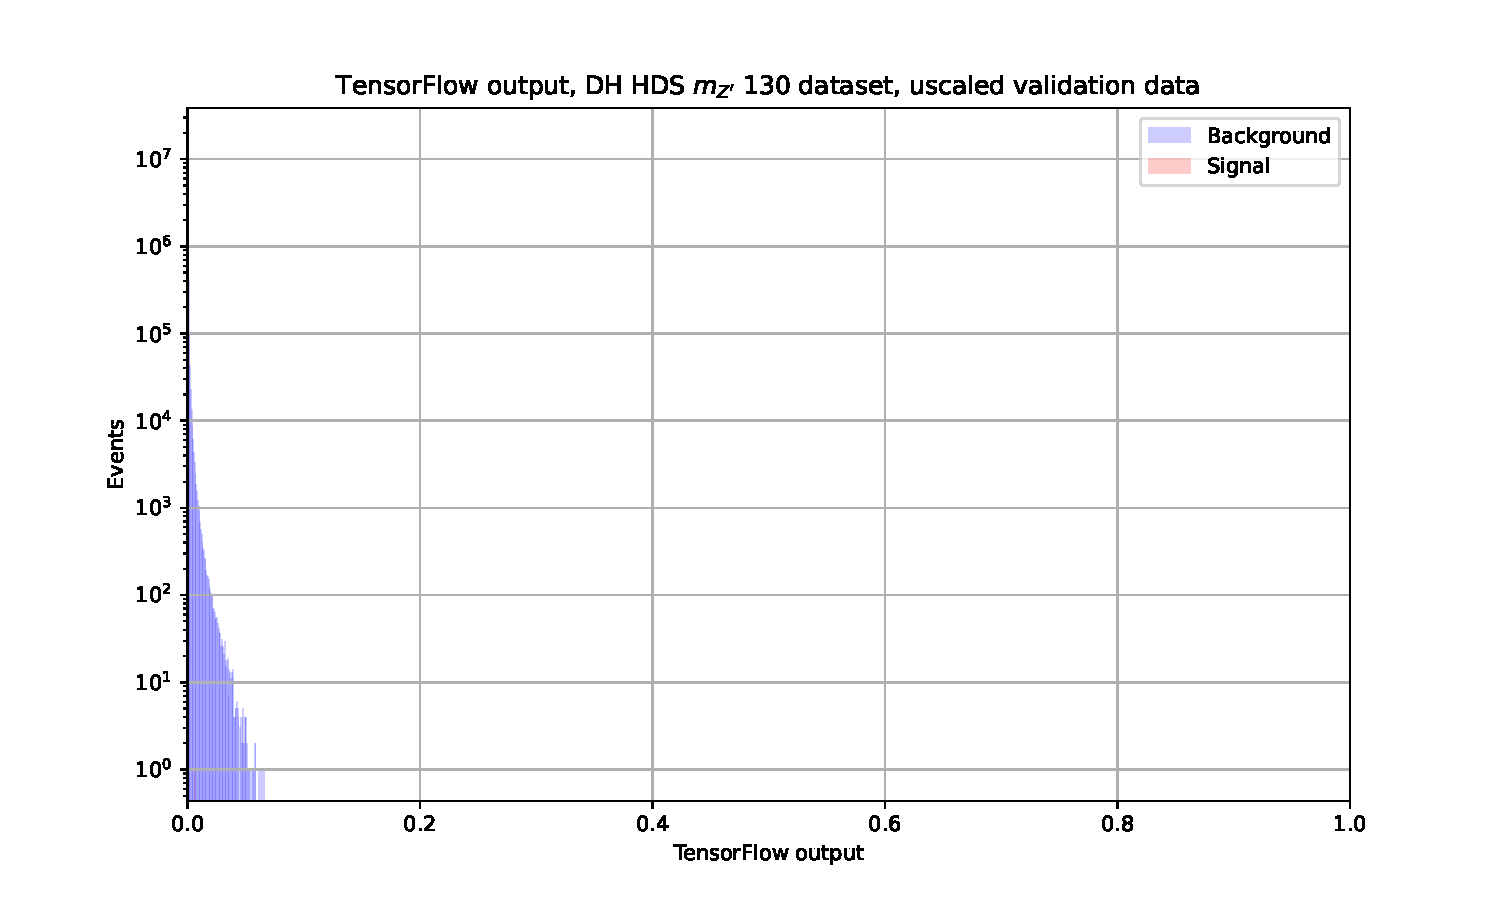
\includegraphics[width=1\textwidth]{DH_HDS_mZp_130/VAL_unscaled.pdf}
        \caption{NN prediction of DH HDS $m_{Z'}$ = 130 GeV}\label{fig:MC_EVT_SIG_DH_HDS_130}
     \end{subfigure}
     \hfill
     \begin{subfigure}[b]{0.49\textwidth}
        \centering
        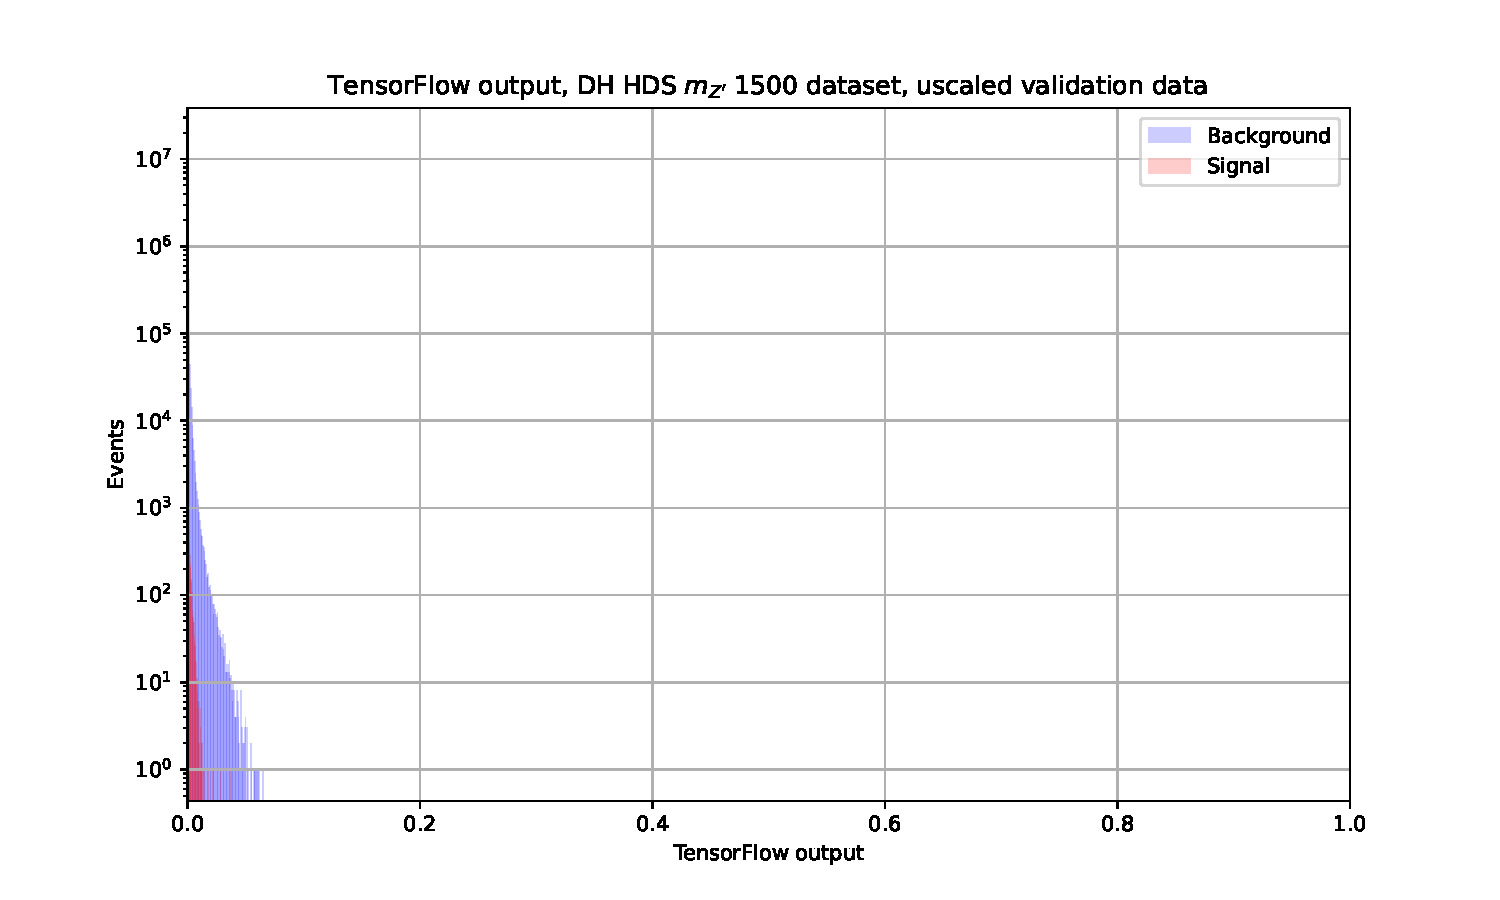
\includegraphics[width=1\textwidth]{DH_HDS_mZp_1500/VAL_unscaled.pdf}
        \caption{NN prediction of DH HDS $m_{Z'}$ = 1500 GeV}\label{fig:MC_EVT_SIG_DH_HDS_1500}
     \end{subfigure}
     \caption{NN prediction when weighting the signal with the raw event ratio.}\label{fig:MC_EVT_SIG_DH_HDS}
\end{figure}
\graphicspath{{../../../Plots/TESTING/NeuralNetwork/BALANCED_WEIGHTING/MC_WGT_BKG_DOWN/}}
\begin{figure}[!ht]
	\centering
	\begin{subfigure}[b]{0.49\textwidth}
        \centering
        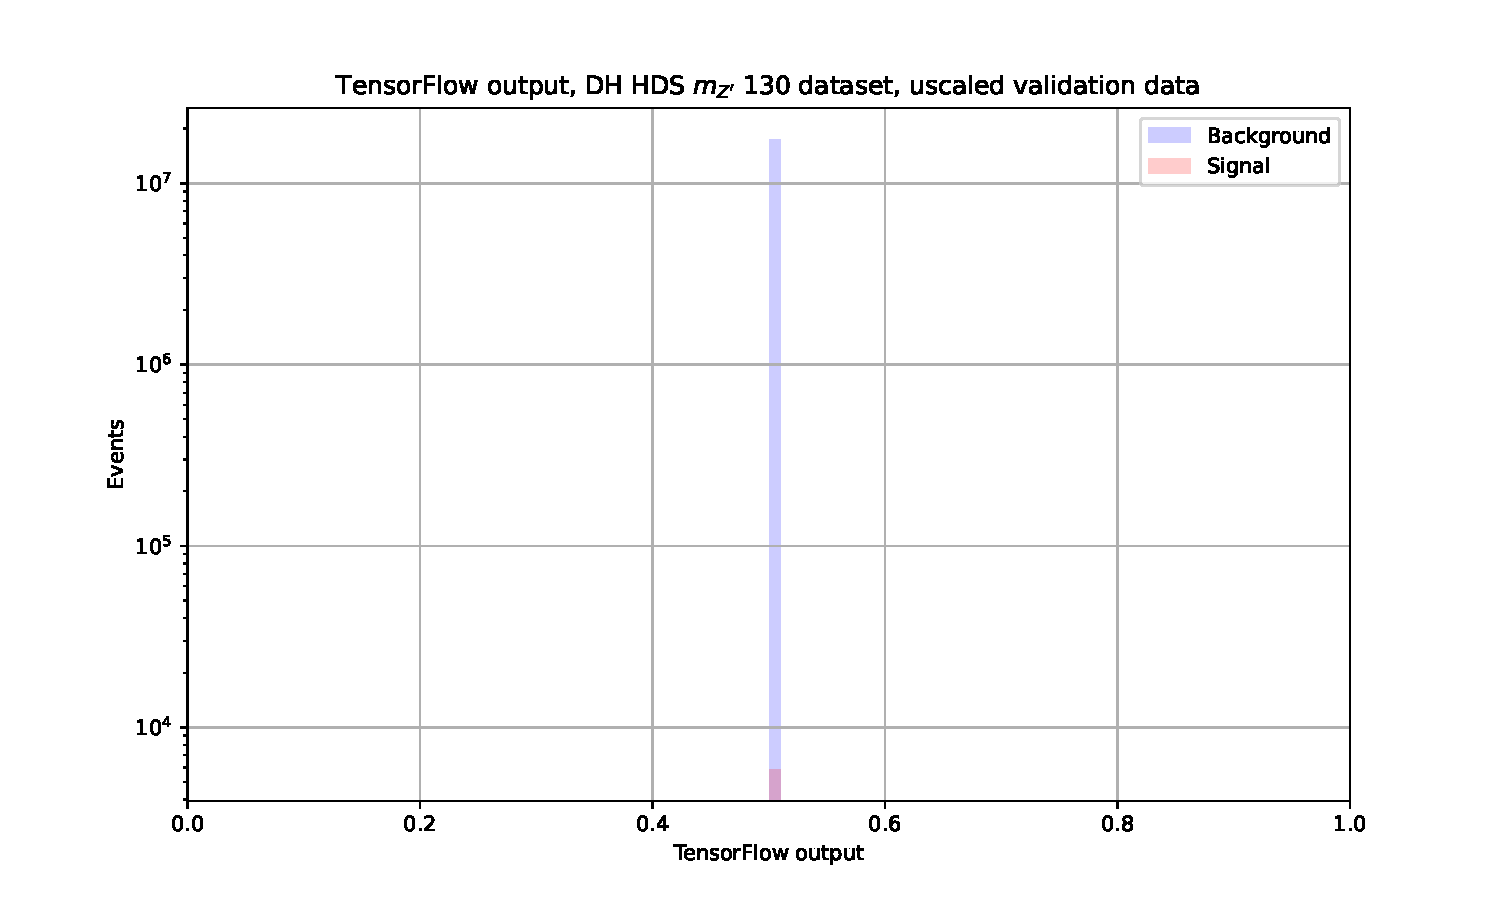
\includegraphics[width=1\textwidth]{DH_HDS_mZp_130/VAL_unscaled.pdf}
        \caption{NN prediction of DH HDS $m_{Z'}$ = 130 GeV}\label{fig:MC_WGT_BKG_DH_HDS_130}
     \end{subfigure}
     \hfill
     \begin{subfigure}[b]{0.49\textwidth}
        \centering
        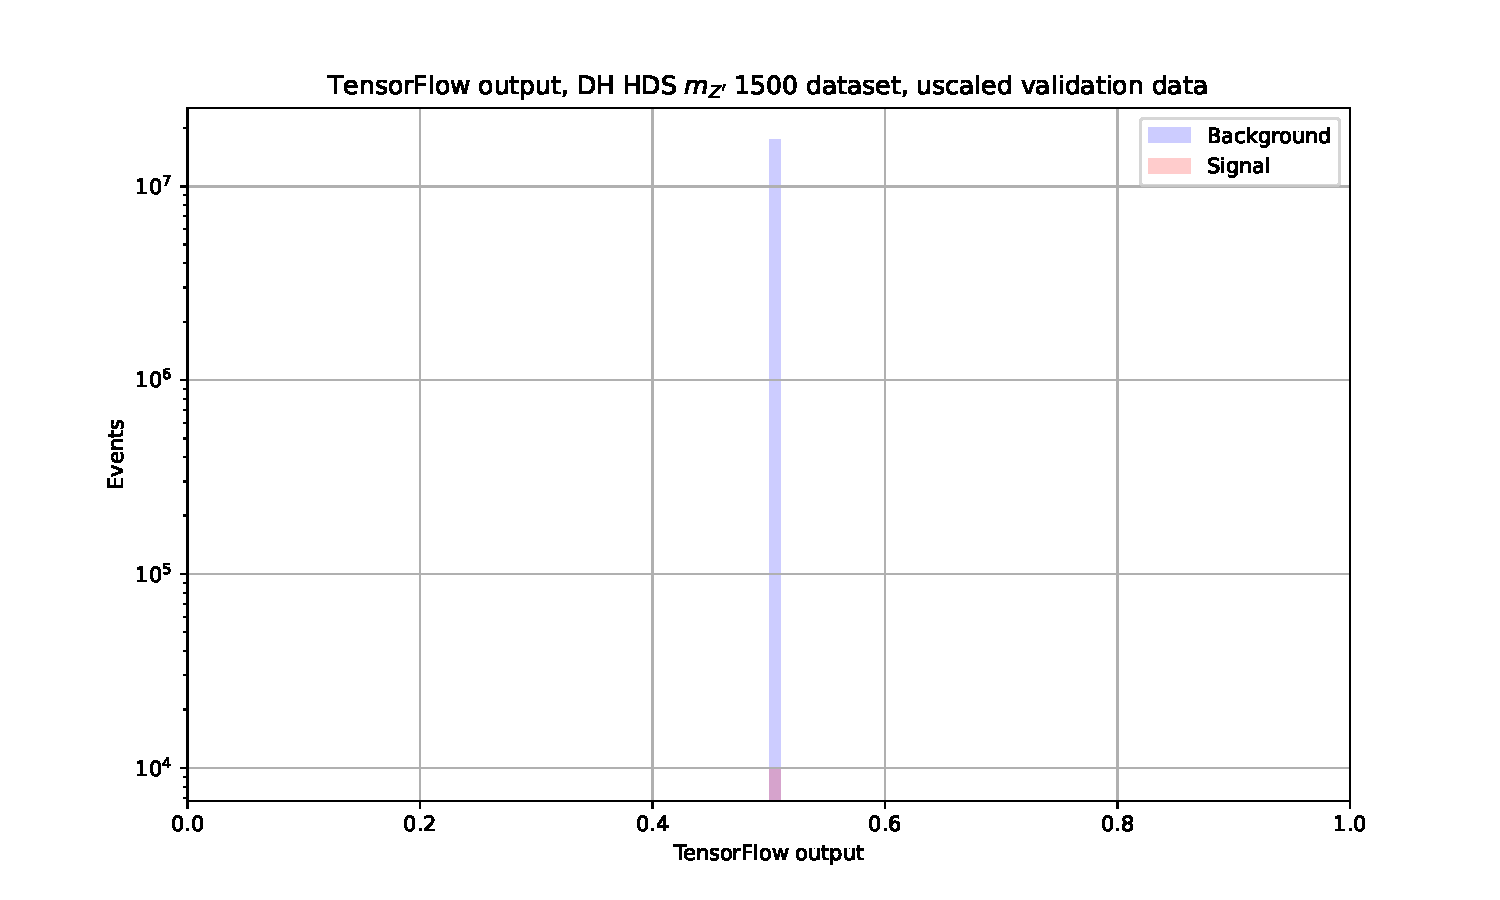
\includegraphics[width=1\textwidth]{DH_HDS_mZp_1500/VAL_unscaled.pdf}
        \caption{NN prediction of DH HDS $m_{Z'}$ = 1500 GeV}\label{fig:MC_WGT_BKG_DH_HDS_1500}
     \end{subfigure}
     \caption{NN prediction when weighting the background with the SOW ratio.}\label{fig:MC_WGT_BKG_DH_HDS}
\end{figure}
\graphicspath{{../../../Plots/TESTING/NeuralNetwork/BALANCED_WEIGHTING/MC_EVENTS_BKG_DOWN/}}
\begin{figure}[!ht]
	\centering
	\begin{subfigure}[b]{0.49\textwidth}
        \centering
        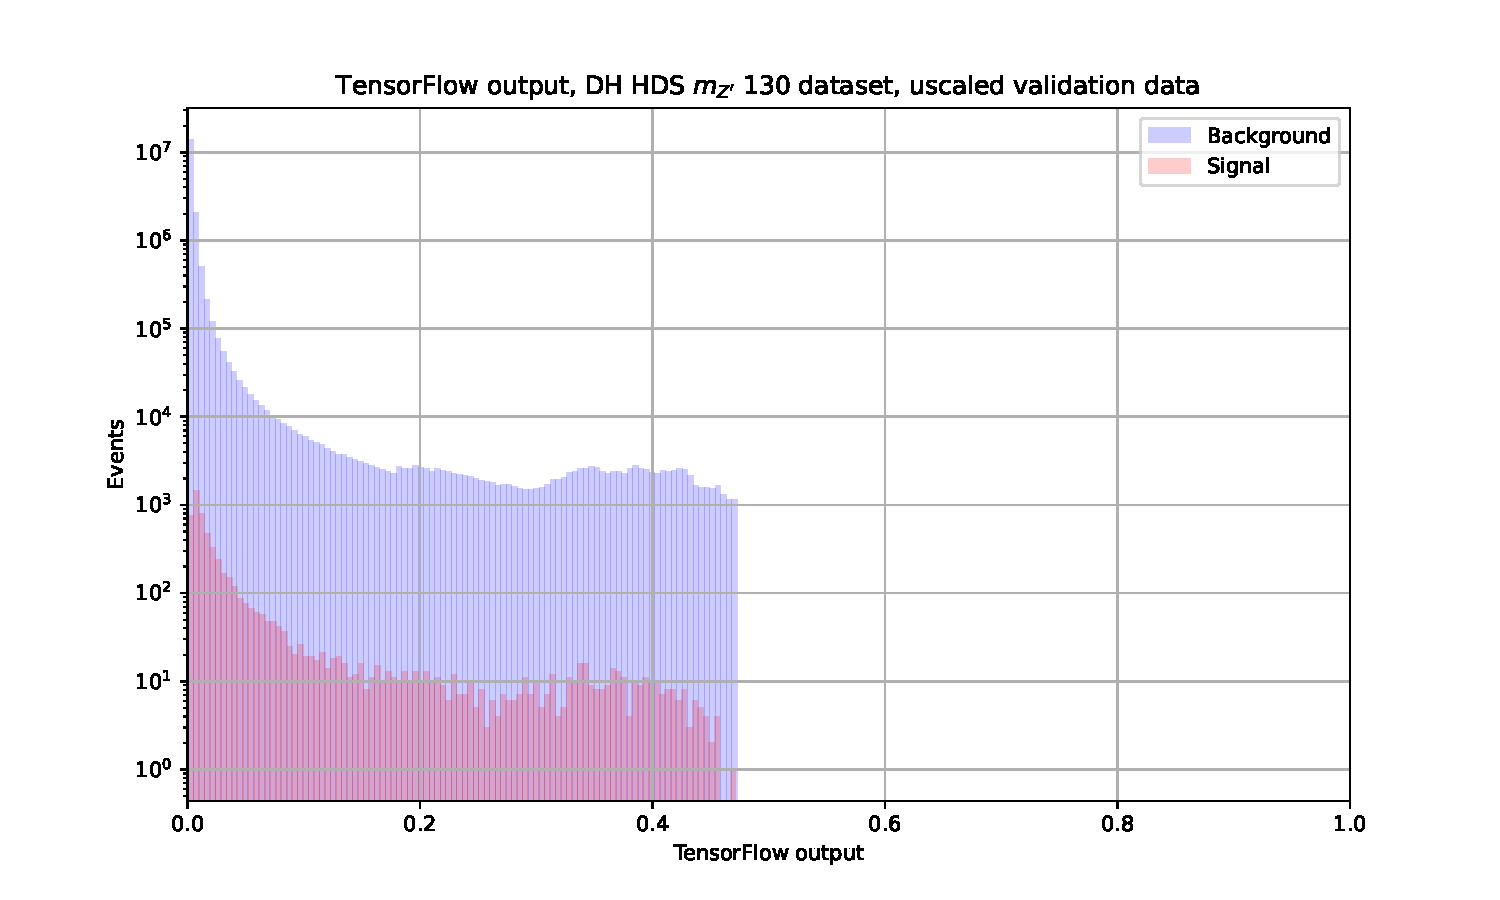
\includegraphics[width=1\textwidth]{DH_HDS_mZp_130/VAL_unscaled.pdf}
        \caption{NN prediction of DH HDS $m_{Z'}$ = 130 GeV}\label{fig:MC_EVT_BKG_DH_HDS_130}
     \end{subfigure}
     \hfill
     \begin{subfigure}[b]{0.49\textwidth}
        \centering
        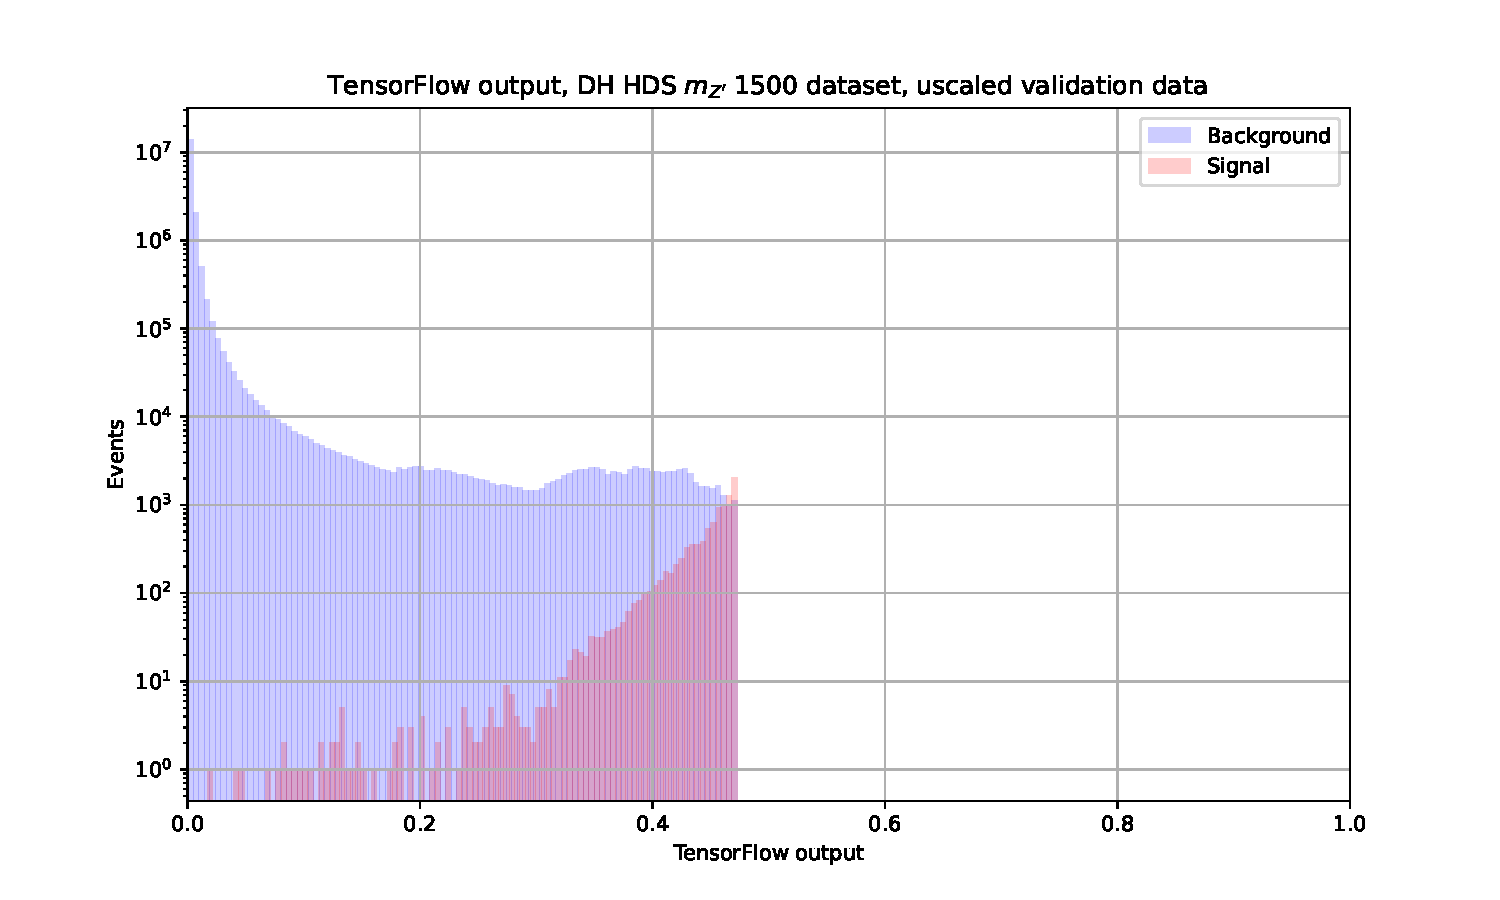
\includegraphics[width=1\textwidth]{DH_HDS_mZp_1500/VAL_unscaled.pdf}
        \caption{NN prediction of DH HDS $m_{Z'}$ = 1500 GeV}\label{fig:MC_EVT_BKG_DH_HDS_1500}
     \end{subfigure}
     \caption{NN prediction when weighting the bacgkround with the raw event ratio.}\label{fig:MC_EVT_BKG_DH_HDS}
\end{figure}
\clearpage 
As we can see almost every way of doing this balanced weighting gives poor results. The only one that seems to work is when we we scale up the MC weights with the ratio between the SOW of the bacgkround over signal, however it does not seem to learn the model with lower mass better compared to how it learned the model with higher mass. It seems to have generally learned both models better, which might be a hint that it learns other models worse, i.e. EFT models with much lower cross section.\\ 
If we now compare the correctly scaled validation plots of DH HDS $m_{Z'}$ = 130 GeV.
\graphicspath{{../../../Plots/TESTING/NeuralNetwork/BALANCED_WEIGHTING/MC_WGT_SIG_UP/}}
\begin{figure}[!ht]
	\centering
	\begin{subfigure}[b]{0.49\textwidth}
        \centering
        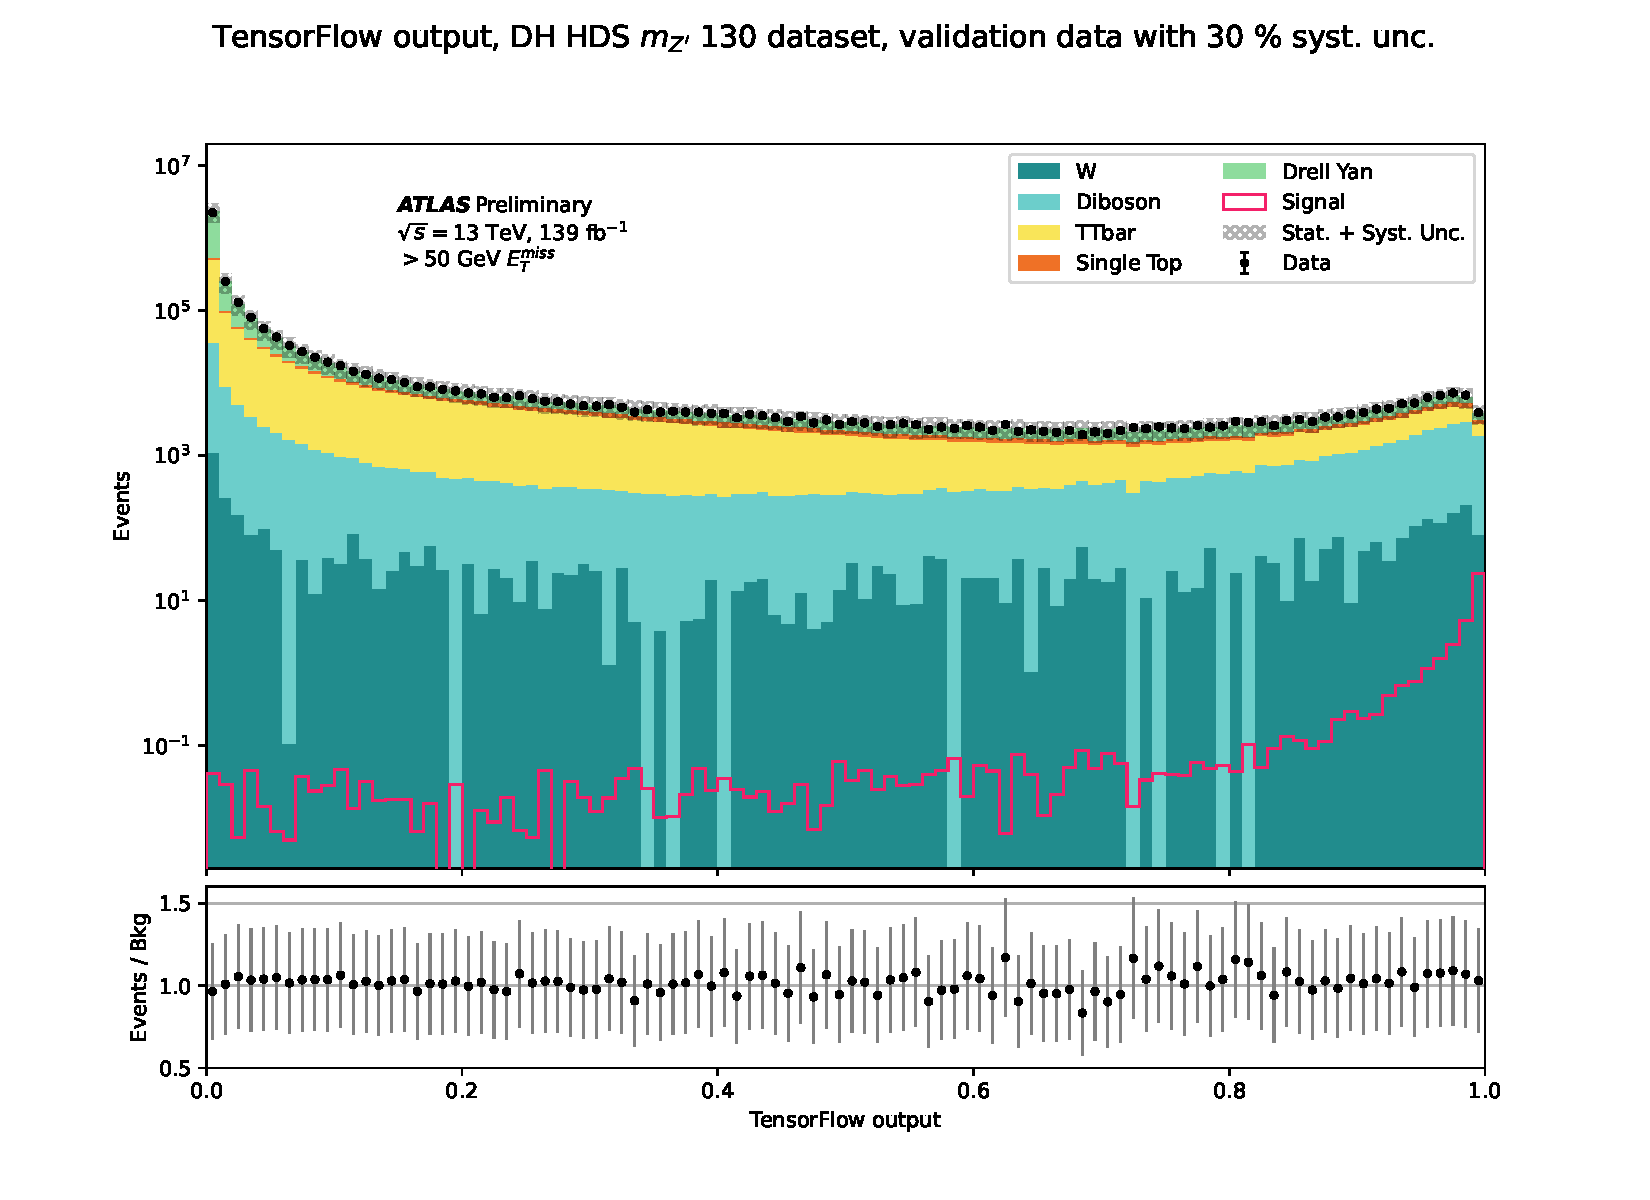
\includegraphics[width=1\textwidth]{DH_HDS_mZp_130/VAL.pdf}
        \caption{MC weights + scaling signal up with SOW ratio}%\label{fig:MC_EVT_BKG_DH_HDS_130}
     \end{subfigure}
     \hfill\graphicspath{{../../../Plots/TESTING/NeuralNetwork/BALANCED_WEIGHTING/ONLY_BALANCE_MC_EVENTS_BKG_DOWN/}}
     \begin{subfigure}[b]{0.49\textwidth}
        \centering
        \includegraphics[width=1\textwidth]{DH_HDS_mZp_130/VAL.pdf}
        \caption{Only using raw MC events weigh down bacgkround}%\label{fig:MC_EVT_BKG_DH_HDS_1500}
     \end{subfigure}
   \hfill\graphicspath{{../../../Plots/TESTING/NeuralNetwork/BALANCED_WEIGHTING/MC_WGT_SIG_UP/}}
   \begin{subfigure}[b]{0.49\textwidth}
      \centering
      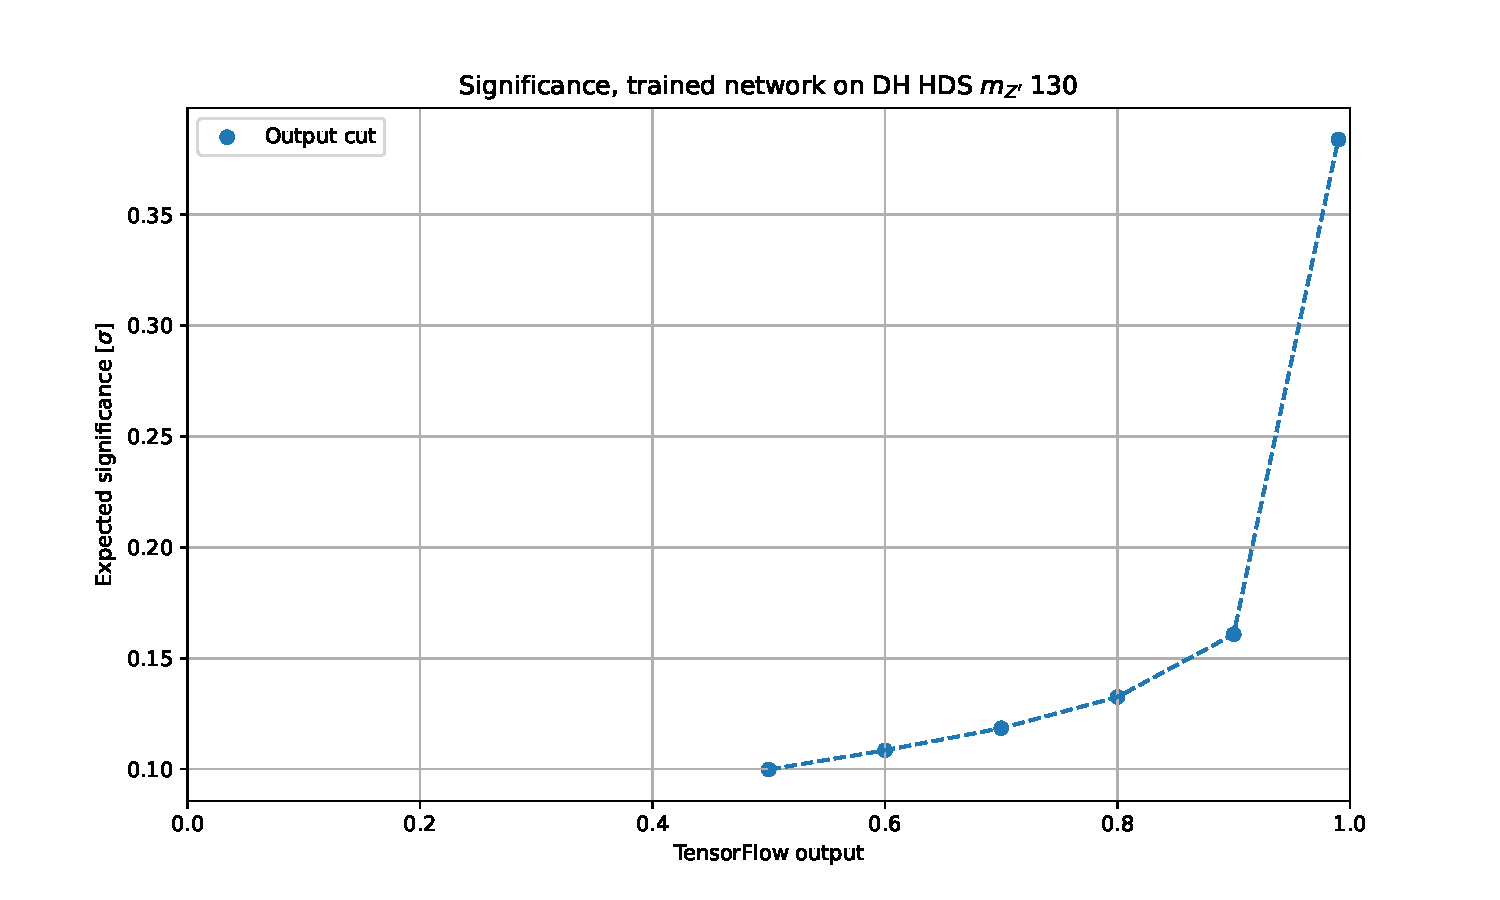
\includegraphics[width=1\textwidth]{DH_HDS_mZp_130/EXP_SIG.pdf}
      \caption{The expected significance of a)}%\label{fig:MC_EVT_BKG_DH_HDS_130}
   \end{subfigure}
   \hfill\graphicspath{{../../../Plots/TESTING/NeuralNetwork/BALANCED_WEIGHTING/ONLY_BALANCE_MC_EVENTS_BKG_DOWN/}}
   \begin{subfigure}[b]{0.49\textwidth}
      \centering
      \includegraphics[width=1\textwidth]{DH_HDS_mZp_130/EXP_SIG.pdf}
      \caption{The expected significance of b)}%\label{fig:MC_EVT_BKG_DH_HDS_1500}
   \end{subfigure}
     \caption{Comparison of the best balanced weighting method to the weighting method of the previous section. Figure a) and b) show the validation data of both cases, c) and d) show the expected significance of the validation plots when making a cut on the output. }%\label{fig:MC_EVT_BKG_DH_HDS}
\end{figure}
\\From this we can see that the the network that trained when balancing the data is better at classifying the DH HDS $m_{Z'}$ = 130 GeV model correctly as signal than the other network. We also observe that it wrongly classifies more background as signal than the other network, but even if this is the case the expected significance is greater in the new network.
The reason that the new network wrongly classifies more background as signal might be becuse I utilized the same hyperparameters when training both newtworks, when it might be better to use different hyperparameters on each. 
Another thing that might be of significance is that I used the ratio of the training set, it might make a difference (better or worse) to use the ratio of the full dataset when training as this is more general. Since the ratio most likely differs for the training and testing set. \textit{\textbf{Both of this options are up to discussion to further pursue. As well as if this appreoach is worth pursuing if it only learns the models with higher cross section.}}


\clearpage

\graphicspath{{../../figures/}}

\section{XGBoost Training}
For XGBoost there is a different problem when it comes to weights. XGBoost has a variable called \verb|scale_pos_weight| where we can help the network deal with unbalanced data, such as the one we have. Thus we can use the \textit{real} weights that are calculated in the MC generators, except not really, XGBoost does not have to possibility to include negative weights. In this project I have therefore used the absolute value of the weights when training. Other than that there are few complications. 

\section{Pure log}
Some problems that have happened is that I had previously made a Deep Neural Network, using three hidden layers. This is however not optimal as the DM statistics is non existent compared to the SM background. Another big problem I had was that I used small bacth sizes when training the Neural Networks. A batch being a portion of the data which is used when training. The reason we batch is to reduce computational power and divide the task of learning. I had a batch size of around 30,000 MC events pr batch. To remind ourselves of our data size, we have around 90,000,000 MC events, from which roughly 40,000 corresponds to a single DM MC DSID. So when batching we trained the network to recognize DM, when there most likely wasn't a single DM sample in the batch itself... this explain the abrupt end, and peak of backgrounds on the signal region seen in Fig. \ref{fig:NN_EXP_SIG:uu}. Thankfully, since I have the supercomputer \verb|hepp03| available I could increase the batch size to a massive amount such as $2^24$ which gives roughly 16 million MC events pr bacth. This is the highest the GPU of the supercomputer can handle!\\
\\With this fixed there was still a big problem, the expected significance of both NN's and XGB is at best half of what a very rough cut and count gives. As mentioned in section 5.1.2, we can split the data in different forms. While splitting it pr DSID works with one hidden layer now it doesn't make much physical sense to do it the way I'm currently doing it when looking at the Z' DM models, since the DM MC samples are splitted into $ee$ and $\mu\mu$ final states. However if we train the network on either final state we are removing the model independent part of the plan (although this increases the significance!). The plan fowards so far is to combine the final states of the Z' DM models as long as they only differ in final lepton state. And compare the significance of these to a statistically combined significance of cut and count.\\
\\One last thing to add as to why the significance might be so much lower for our networks is that I have not yet done a grid search for the best hyperparameters and loss functions. Doing this with XGBoost is easy, but there is a memory leak in the codebase of TensorFlow that makes the process tedious... This is where I am at in the present time, as well as waiting for more DM data.

\section{Comparison to cut and count}
Testing three models using the classical data analysis way we apply cuts to kinematic variables and try to isolate the signal from the background to then calculated the expected significance. The three models I chose to test are all High Dark Sector models with $m_{Z'}=130$GeV. They are a Light Vector (LV), Dark Higgs (DH) and Effective Field Theory (EFT) models. The cuts I made on these are shown in Table \ref{tab:cuts}.
\begin{table}[!h]
    \centering
    \begin{tabular}{l|r}\midrule\midrule
                                & Cut\\\midrule
         $E_T^{miss}/\sigma$    & > 10      \\
         $m_T$                  & > 160 GeV \\
         $m_{ll}$               & > 120 GeV \\
         Number of B-jets       & 0         \\
         $m_{T2}$               & > 110 GeV \\\midrule\midrule
    \end{tabular}
    \caption[Cut and count cuts]{Table showcasing the cuts used when doing the cut and count method.}
    \label{tab:cuts}
\end{table}
\\ Since the cross section to find Dark Matter is really small we have to use the low-statistics expected significance formula to find the closest to correct significance. The formula is
\begin{equation}\label{eq:low_stat_Z}
    Z = \sqrt{2\left[(s + b)\ln(1 + \frac{s}{b}) - s \right]}
\end{equation}
Where $s$ is the number of signal events and $b$ is the number of background events. Using this we get the results shown in Table \ref{tab:cutsigee} for the electron channel and Table \ref{tab:cutsiguu} for the muon channel. Also included on the tables are the number of events. One thing worth mentioning is that when adding another cut on the maximum invariant mass increases the significance. The significance for LV on the electron channel was at $1.2\sigma$ when adding a cut stating that $m_{ll}<150$ GeV. This makes sense since the models in question all have a $m_{Z'}=130$GeV. This cut was not added since we do not want to put a cap on the mass of the propagator, as we don't know what the real mass is.
\begin{table}[!h]
    \centering
    \begin{tabular}{l|c|c|c|r}\midrule\midrule
                                          & LV  & DH  & EFT & Background \\\midrule
         Events before cuts               & 15  & 20  & 0   & 1,256,624    \\
         Events after cuts                & 4   & 6   & 0   & 117 \\
         Expected significance [$\sigma$] & 0.4 & 0.6 & 0   & \\\midrule\midrule
    \end{tabular}
    \caption[Cut and count significance ee]{Table showcasing the result of the cut and count method for the electron channel.}
    \label{tab:cutsigee}
\end{table}
\begin{table}[!h]
    \centering
    \begin{tabular}{l|c|c|c|r}\midrule\midrule
                                          & LV  & DH  & EFT & Background \\\midrule
         Events before cuts               & 14  & 19  & 0   & 1,626,098    \\
         Events after cuts                & 3   & 5   & 0   & 108 \\
         Expected significance [$\sigma$] & 0.36 & 0.51 & 0   & \\\midrule\midrule
    \end{tabular}
    \caption[Cut and count significance uu]{Table showcasing the result of the cut and count method for the muon channel.}
    \label{tab:cutsiguu}
\end{table}
\\If we were to compare these results with what our NN and BDT that trained on the full dataset we see that we can calculate the expected significance in different locations for the validation plots. Testing on the networks that trained using the data scientist method on the full DM dataset we get the results shown in Figure \ref{fig:XGB_SIG_FULL} for XGBoost and Figure \ref{fig:NN_SIG_FULL} for the Neural Network.
\begin{figure}[!ht]
	\centering
	\begin{subfigure}[b]{0.8\textwidth}
        \centering
        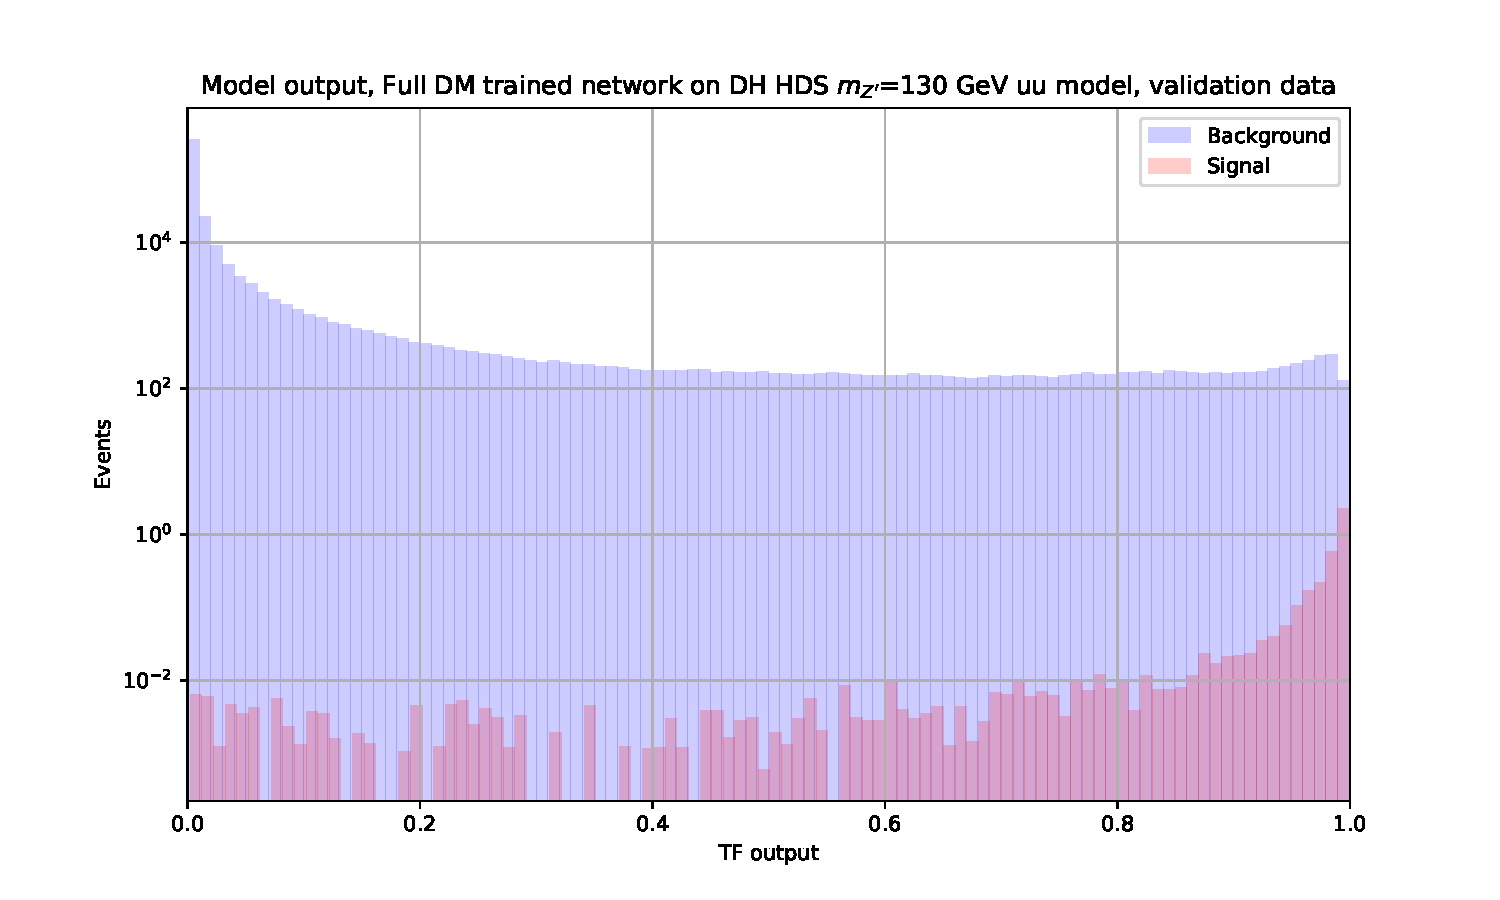
\includegraphics[width=1\textwidth]{XGB_VAL_uu.pdf}
        \caption{Validation plot.}\label{fig:XGB_VAL_UU}
     \end{subfigure}
     \hfill
     \begin{subfigure}[b]{0.8\textwidth}
        \centering
        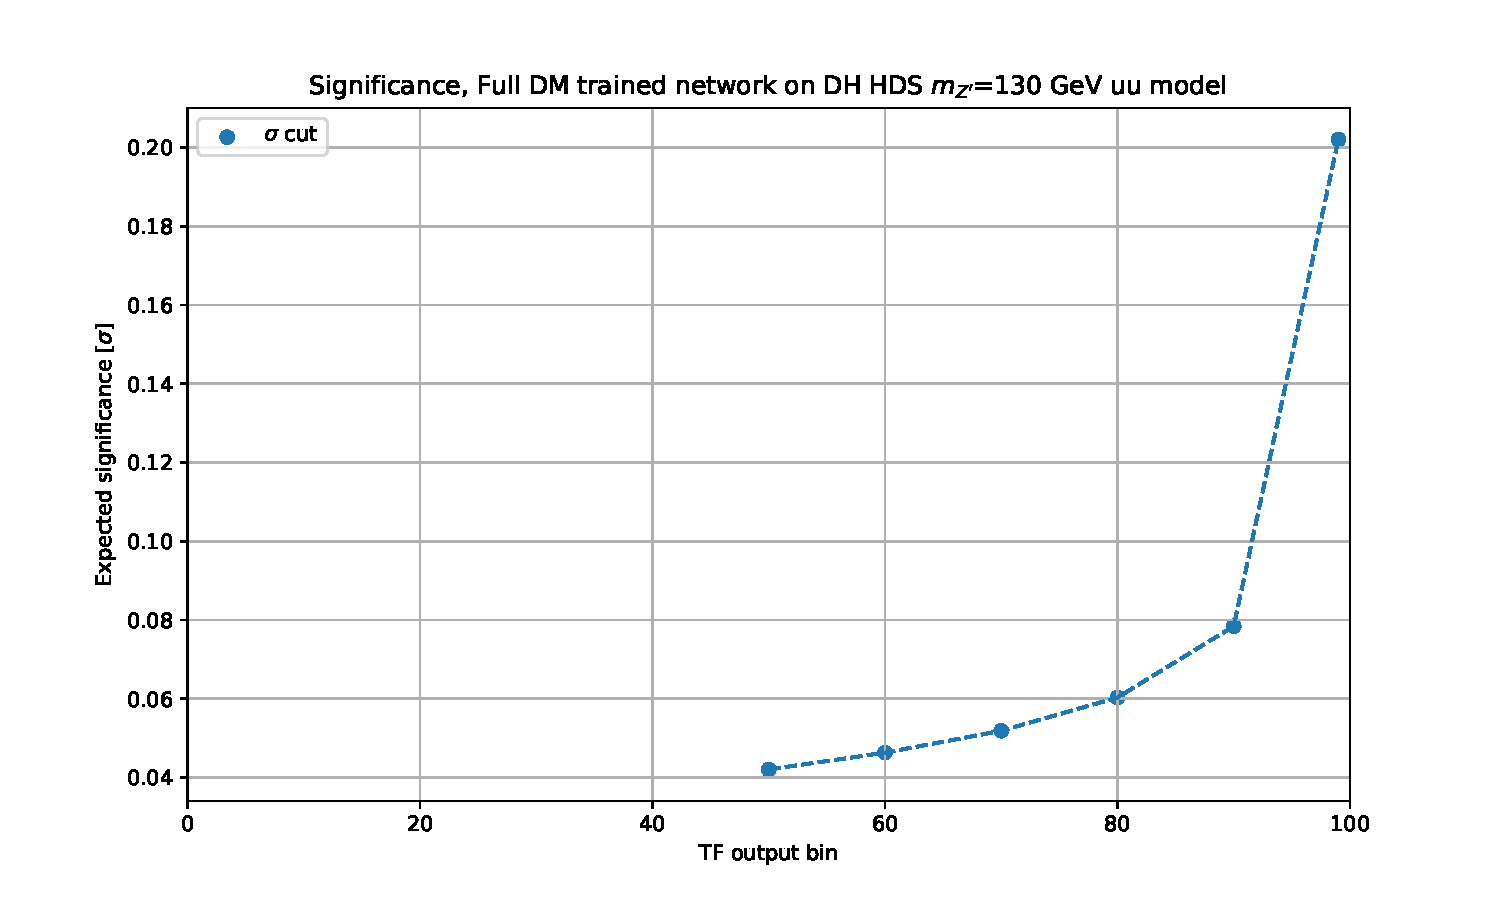
\includegraphics[width=1\textwidth]{XGB_EXP_SIG_uu.pdf}
        \caption{Expected significance when looking at bins and forth.}\label{fig:XGB_EXP_SIG:uu}
     \end{subfigure}
	\caption{Expected significance of XGBoost when trained on the Full DM dataset for the DH HDS $m_{Z'}$ = 130 GeV muon model.}\label{fig:XGB_SIG_FULL}
\end{figure}
\begin{figure}[!ht]
	\centering
	\begin{subfigure}[b]{0.8\textwidth}
        \centering
        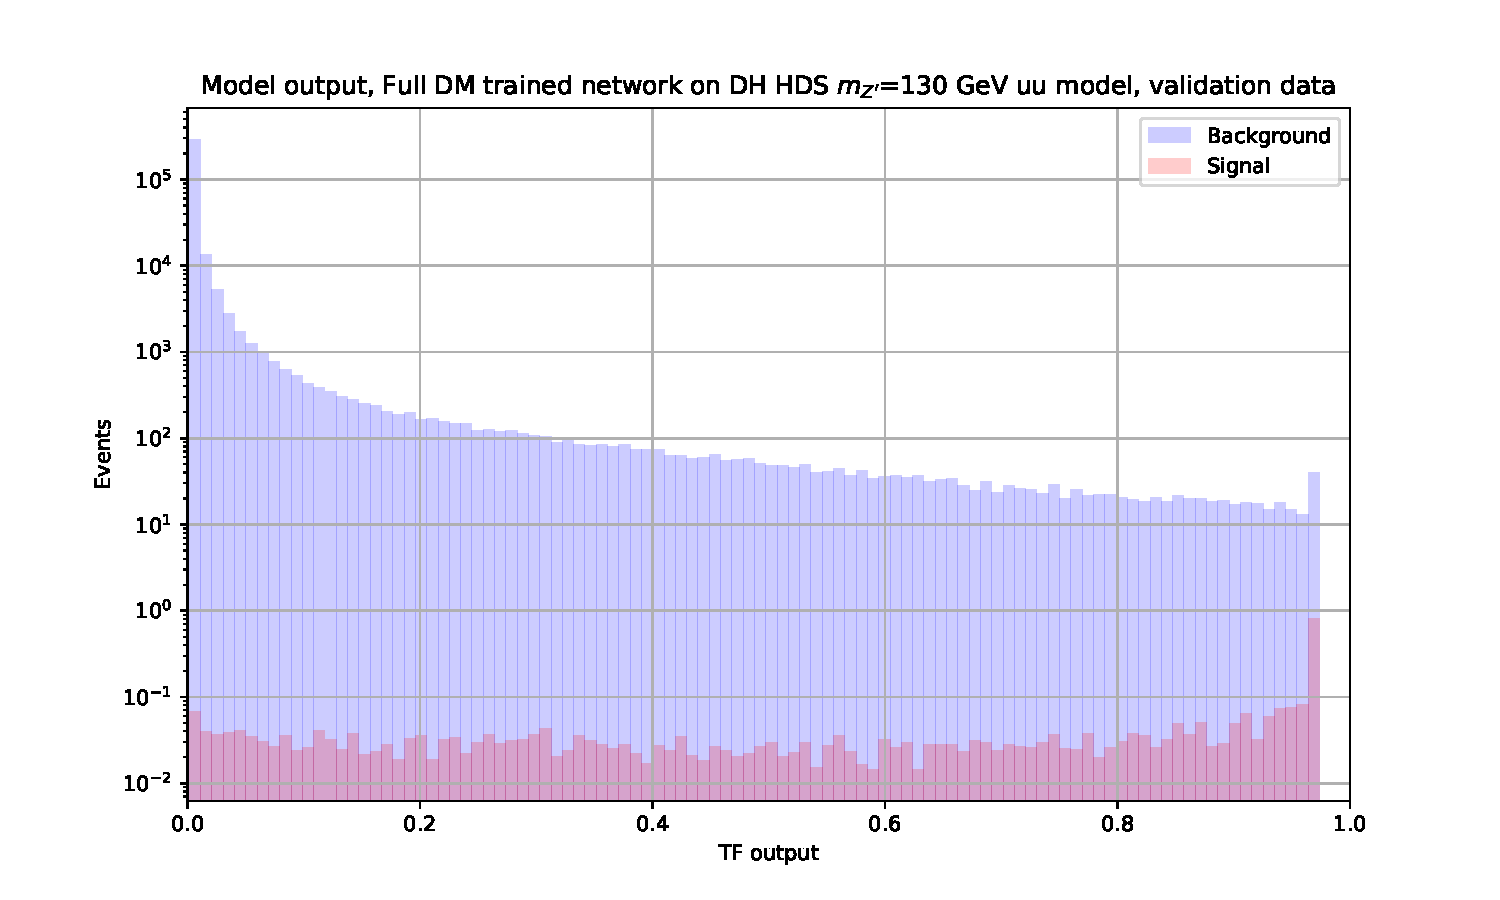
\includegraphics[width=1\textwidth]{NN_VAL_uu.pdf}
        \caption{Validation plot.}\label{fig:NN_VAL_UU}
     \end{subfigure}
     \hfill
     \begin{subfigure}[b]{0.8\textwidth}
        \centering
        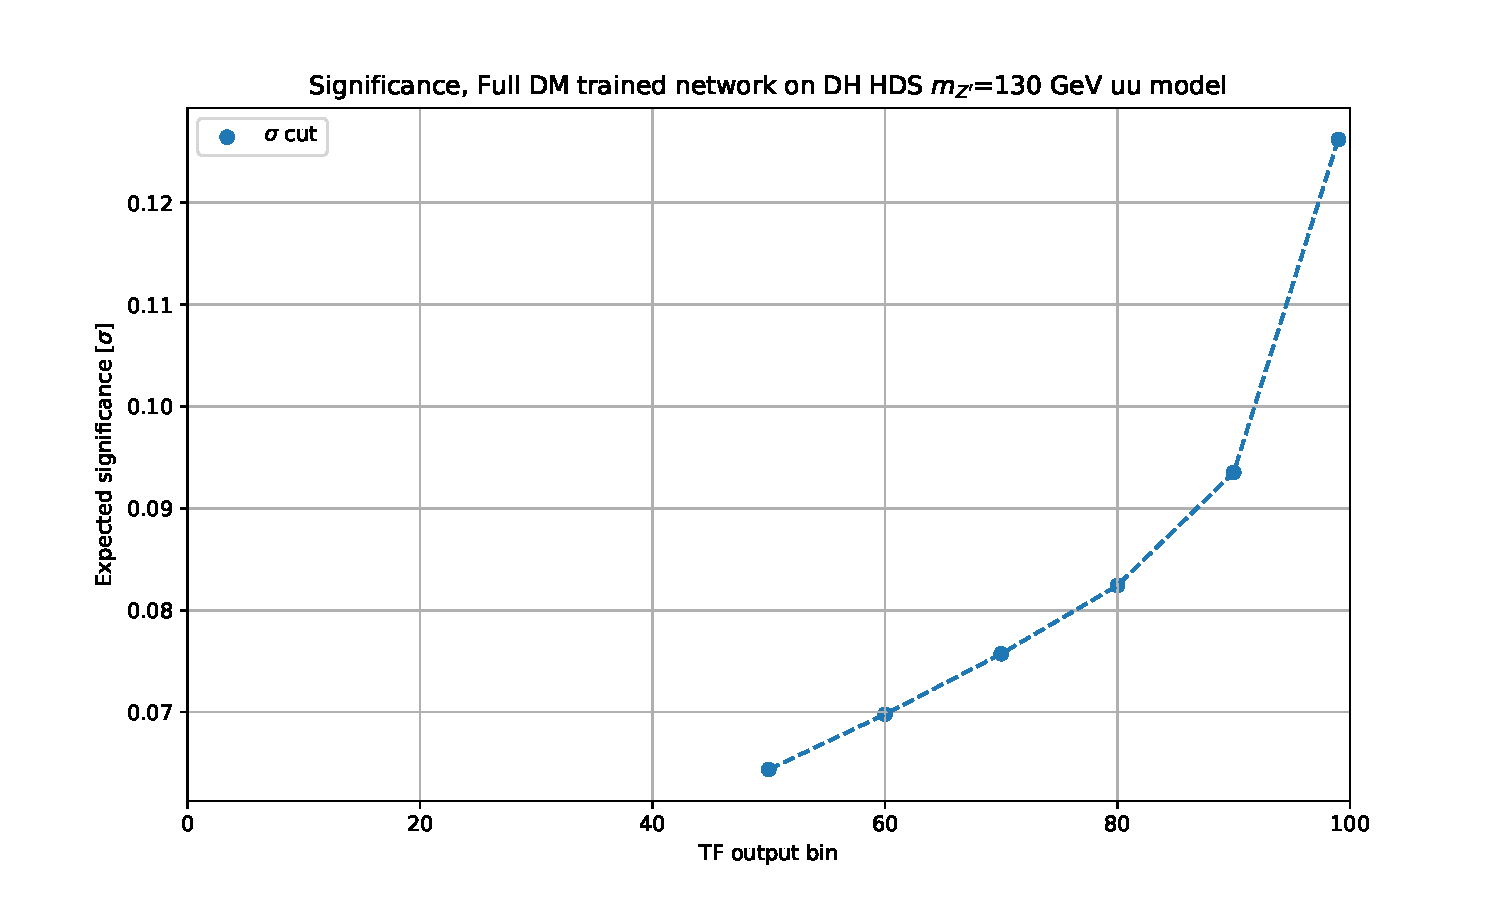
\includegraphics[width=1\textwidth]{NN_EXP_SIG_uu.pdf}
        \caption{Expected significance when looking at bins and forth.}\label{fig:NN_EXP_SIG:uu}
     \end{subfigure}
	\caption{Expected significance of the Neural Network when trained on the Full DM dataset for the DH HDS $m_{Z'}$ = 130 GeV muon model.}\label{fig:NN_SIG_FULL}
\end{figure}
\clearpage As we can see the expected significance is lower using ML than a rough cut and count. My theory for why this is the case is because we are testing just \textit{\textbf{one}} sample out of 154 different ones that are included for the three different theories I have acquired so far. And the ML networks shown above have both trained on a dataset including all 154 DM samples. The models that I tested might also not have been one of the "important" models the network learned from. Thus if I were to train the network individually based on the theory it might give better results.

\end{document}